%
% exemplo genérico de uso da classe iiufrgs.cls
% $Id: iiufrgs.tex,v 1.1.1.1 2005/01/18 23:54:42 avila Exp $
%
% This is an example file and is hereby explicitly put in the
% public domain.
%
\documentclass[ecp,tc, english]{iiufrgs}
% Para usar o modelo, deve-se informar o programa e o tipo de documento.
% Programas :
%   * cic       -- Graduação em Ciência da Computação
%   * ecp       -- Graduação em Ciência da Computação
%   * ppgc      -- Programa de Pós Graduação em Computação
%   * pgmigro   -- Programa de Pós Graduação em Microeletrônica
%   
% Tipos de Documento:
%   * tc                -- Trabalhos de Conclusão (apenas cic e ecp)
%   * diss ou mestrado  -- Dissertações de Mestrado (ppgc e pgmicro)
%   * tese ou doutorado -- Teses de Doutorado (ppgc e pgmicro)
%   * ti                -- Trabalho Individual (ppgc e pgmicro)
% 
% Outras Opções:
%   * english    -- para textos em inglês
%   * openright  -- Força início de capítulos em páginas ímpares (padrão da
%                   biblioteca)
%   * oneside    -- Desliga frente-e-verso
%   * nominatalocal -- Lê os dados da nominata do arquivo nominatalocal.def


% Use unicode
\usepackage[utf8]{inputenc}   % pacote para acentuação
\usepackage{varioref}
\usepackage{amsmath}
% Necessário para incluir figuras
\usepackage{graphicx}           % pacote para importar figuras
\usepackage{caption}
\usepackage{subcaption}
\usepackage{multirow}
\usepackage[normalem]{ulem}
\useunder{\uline}{\ul}{}

\newcommand*\xor{\mathbin{\oplus}}

\usepackage{times}              % pacote para usar fonte Adobe Times
% \usepackage{palatino}
% \usepackage{mathptmx}          % p/ usar fonte Adobe Times nas fórmulas

\usepackage[alf,abnt-emphasize=bf]{abntex2cite}	% pacote para usar citações abnt

%
% Informações gerais
%
\title{Evaluation of Variability using Schmitt Trigger on Full Adders Layout}

\author{Moraes}{Leonardo Barlette de}
% alguns documentos podem ter varios autores:
%\author{Flaumann}{Frida Gutenberg}
%\author{Flaumann}{Klaus Gutenberg}

% orientador e co-orientador são opcionais (não diga isso pra eles :))
\advisor[Prof.~Dr.]{Reis}{Ricardo}
%\coadvisor[Prof.~Dr.]{Meinhardt}{Cristina}
\coadvisor[Prof.~Dr]{Zimpeck}{Alexandra Lackmann}

% a data deve ser a da defesa; se nao especificada, são gerados
% mes e ano correntes
\date{July}{2018}

% o local de realização do trabalho pode ser especificado (ex. para TCs)
% com o comando \location:
%\location{Itaquaquecetuba}{SP}

% itens individuais da nominata podem ser redefinidos com os comandos
% abaixo:
% \renewcommand{\nominataReit}{Prof\textsuperscript{a}.~Wrana Maria Panizzi}
% \renewcommand{\nominataReitname}{Reitora}
% \renewcommand{\nominataPRE}{Prof.~Jos{\'e} Carlos Ferraz Hennemann}
% \renewcommand{\nominataPREname}{Pr{\'o}-Reitor de Ensino}
% \renewcommand{\nominataPRAPG}{Prof\textsuperscript{a}.~Joc{\'e}lia Grazia}
% \renewcommand{\nominataPRAPGname}{Pr{\'o}-Reitora Adjunta de P{\'o}s-Gradua{\c{c}}{\~a}o}
% \renewcommand{\nominataDir}{Prof.~Philippe Olivier Alexandre Navaux}
% \renewcommand{\nominataDirname}{Diretor do Instituto de Inform{\'a}tica}
% \renewcommand{\nominataCoord}{Prof.~Carlos Alberto Heuser}
% \renewcommand{\nominataCoordname}{Coordenador do PPGC}
% \renewcommand{\nominataBibchefe}{Beatriz Regina Bastos Haro}
% \renewcommand{\nominataBibchefename}{Bibliotec{\'a}ria-chefe do Instituto de Inform{\'a}tica}
% \renewcommand{\nominataChefeINA}{Prof.~Jos{\'e} Valdeni de Lima}
% \renewcommand{\nominataChefeINAname}{Chefe do \deptINA}
% \renewcommand{\nominataChefeINT}{Prof.~Leila Ribeiro}
% \renewcommand{\nominataChefeINTname}{Chefe do \deptINT}

% A seguir são apresentados comandos específicos para alguns
% tipos de documentos.

% Relatório de Pesquisa [rp]:
% \rp{123}             % numero do rp
% \financ{CNPq, CAPES} % orgaos financiadores

% Trabalho Individual [ti]:
% \ti{123}     % numero do TI
% \ti[II]{456} % no caso de ser o segundo TI

% Monografias de Especialização [espec]:
% \espec{Redes e Sistemas Distribuídos}      % nome do curso
% \coord[Profa.~Dra.]{Weber}{Taisy da Silva} % coordenador do curso
% \dept{INA}                                 % departamento relacionado

%
% palavras-chave
% iniciar todas com letras minúsculas, exceto no caso de abreviaturas
%
\keyword{formatação eletrônica de documentos}
\keyword{\LaTeX}
\keyword{ABNT}
\keyword{UFRGS}

%
% inicio do documento
%
\begin{document}

% folha de rosto
% às vezes é necessário redefinir algum comando logo antes de produzir
% a folha de rosto:
% \renewcommand{\coordname}{Coordenadora do Curso}
\maketitle

% dedicatoria
\clearpage
\begin{flushright}
\mbox{}\vfill
{\sffamily\itshape
``If I have seen farther than others,\\
it is because I stood on the shoulders of giants.''\\}
--- \textsc{Sir~Isaac Newton}
\end{flushright}

% agradecimentos
\chapter*{Agradecimentos}
Agradeço ao \LaTeX\ por não ter vírus de macro\ldots



% resumo na língua do documento
\begin{abstract}
    The aggressive technology and voltage scaling which modern digital circuits are facing introduce a higher influence in metrics, as performance and power consumption, due to process variability. To mitigate that, novel techniques are proposed and tested in the literature. This work analyzes the impact on variability robustness using a technique based on the replacement of full adders internal inverters by Schmitt Triggers. Some works point that the given technique helps to improve the variability robustness at the electrical level. Therefore, analysis has been performed at layout level using the 7nm FinFET technology node from ASAP7 library and the technique was applied on four full adder designs. Performance, energy and area are taken into account. Results show up to 64.74\% and 66.6\% improvement in average delay and energy variability robustness, respectively.
\end{abstract}

% resumo na outra língua
% como parametros devem ser passados o titulo e as palavras-chave
% na outra língua, separadas por vírgulas
% \begin{englishabstract}{Using \LaTeX\ to Prepare Documents at II/UFRGS}{Electronic document preparation, \LaTeX, ABNT, UFRGS}
% This document is an example on how to prepare documents at II/UFRGS
% using the \LaTeX\ classes provided by the UTUG\@. At the same time, it
% may serve as a guide for general-purpose commands. \emph{The text in
% the abstract should not contain more than 500~words.}
% \end{englishabstract}

% lista de abreviaturas e siglas
% o parametro deve ser a abreviatura mais longa
\begin{listofabbrv}{SPMD}
        \item[FA] Full Adder
        \item[PVT] Process, Voltage and Temperature
\end{listofabbrv}

% idem para a lista de símbolos
%\begin{listofsymbols}{$\alpha\beta\pi\omega$}
%       \item[$\sum{\frac{a}{b}}$] Somatório do produtório
%       \item[$\alpha\beta\pi\omega$] Fator de inconstância do resultado
%\end{listofsymbols}

% lista de figuras
\listoffigures

% lista de tabelas
\listoftables

% sumario
\tableofcontents

% aqui comeca o texto propriamente dito

% introducao
\chapter{Introduction}
The technology scaling over the years have significantly increased the density of transistors present on chips. Alongside, with the advance over transistor technology, new challenges were introduced due to the scale down, as aging effects, high power consumption due to leakage current and an increase in the sensibility to transient faults due to radiation and process variability \cite{abbas:15}.

The same technology scaling that allowed the increase in transistor density also allowed a voltage scaling due to the shortening of gate dimensions, internal capacitances and resistances. These two combined events contributed to the emergence, growth and current dominance of mobile applications over its counterpart. This new context, introduced a concern for battery lifespan which these applications are dependent \cite{islam:10}. 

The ascending number of mobile applications that depends on highly sophisticated processing schemes with a limited power-supply capability of today’s batteries brings conflicting needs. The need to explore high-performance designs and implementations to meet the speed constraints for real-time applications and, simultaneously, consider low-power design approaches to extend the battery life of portable devices \cite{shoarinejad:03}. 

Due to the new power consumption concern, novel types of logic blocks for chips started being designed for low power. One of the most present logic blocks in computer systems is the Full Adder. It plays a central role in performing general arithmetic operations such as addition, subtraction, division, shift and so on. The full adder operation adds two bits considering the Carry Out value from a less significant stage. It follows the equations \ref{eqn:01} and \ref{eqn:02} with the Truth Table \ref{tab:01}.

\begin{equation}
\label{eqn:01}
\text{Sum} = (A \xor{} B) \xor{} Cin
\end{equation}
\begin{equation}
\label{eqn:02}
\text{Cout} = (A \wedge B) \vee Cin \wedge (A \xor{} B)
\end{equation}

\begin{table}[H]
\centering
\caption{Truth Table of Full Adders}
\label{tab:01}
\begin{tabular}{|c|c|c|c|c|}
\hline
\multicolumn{3}{|c|}{Input} & \multicolumn{2}{c|}{Output} \\ \hline
A       & B      & Cin      & Sum          & Cout         \\ \hline
0       & 0      & 0        & 0            & 0            \\ \hline
0       & 0      & 1        & 1            & 0            \\ \hline
0       & 1      & 0        & 1            & 0            \\ \hline
0       & 1      & 1        & 0            & 1            \\ \hline
1       & 0      & 0        & 1            & 0            \\ \hline
1       & 0      & 1        & 0            & 1            \\ \hline
1       & 1      & 0        & 0            & 1            \\ \hline
1       & 1      & 1        & 1            & 1            \\ \hline
\end{tabular}
\end{table}

Adder cells define the throughput and are employed in the processor’s executive, floating-point, and memory address generation units. Due to its absolute numbers in microprocessors and their part on the critical path of electronic systems, any improvements over adding blocks generates a considerable improvement in the whole system because of the huge influence of power, timing and area characteristics on the system design \cite{shoarinejad:03}.

Moore’s law predicts that the number of transistors per square on integrated circuits will double every year and it has been guiding the industry trending for decades. However, continue with scaling in the bulk CMOS technology has been no straightforward task. At deep nanotechnology nodes, each chip may show different behavior due to process variations during the manufacturing steps. Variations that influence the circuits metrics such as performance and power consumption, hastening the circuit degradation and making it deviate from its correct operation \cite{abbas:15} \cite{nassif:08}. 

In this context, this work employs a technique using Schmitt Trigger (ST) inverters for process variability mitigation on different Full Adder topologies with priority on power consumption variations. Performance, power, and area penalty will be analyzed alongside variability robustness. 

Promising new commercial technologies based on the Fin Field Effect Transistor (FinFET) devices have been introduced to maintain the technology scaling. The process variability impact on those technologies have shown to be less present, although it can not be ignored, being necessary more research concerning the characterization of process variability effect on emerging technologies. 

FinFET technology is built on a Silicon on Insulator (SOI) substrate with a conducting channel that rises above the level of the insulator, creating a thin silicon structure, the gate as shown in Figure \ref{fig:Fig1}. The channel being surrounded from three dimensions by the gate results in a superior control, reduced SCE (short-channel effect) and eliminated RDF (random dopant fluctuation) effect due to the fully depleted channel that causes less sensitivity to process variations \cite{taur2013fundamentals}. 

\begin{figure}[ht]
\centering
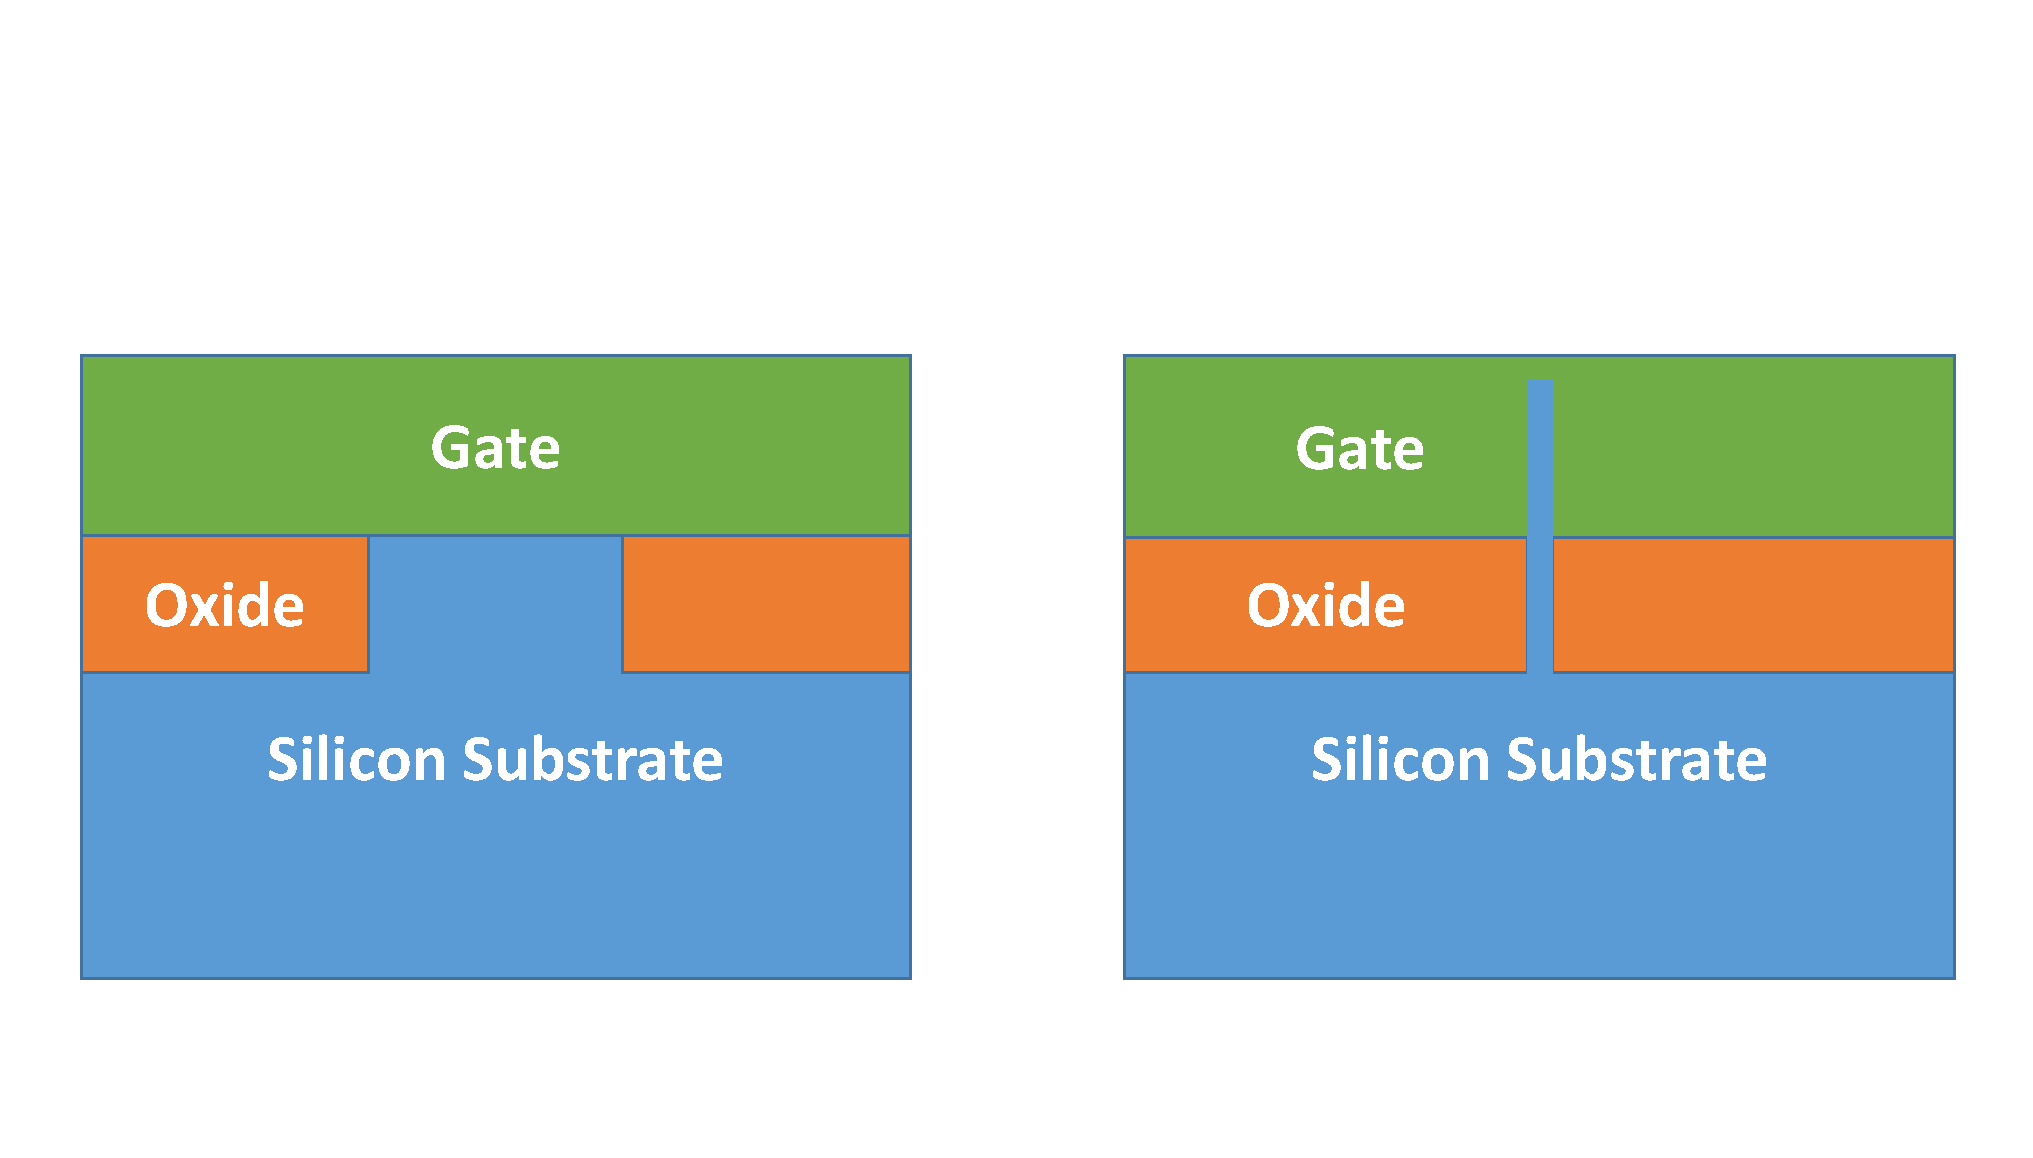
\includegraphics[width=.8\textwidth, trim={0 3cm 0 5cm},clip]{bulkvsfinfet.eps}
\caption{Comparison between Bulk CMOS (left) and FinFET (right) transistors.}
\label{fig:Fig1}
\end{figure}

This work is divided into six further sections: Variability Effects and Mitigation Techniques, with a theoretical foundation about variability. Motivation and Objectives, explaining in more details this work’s objective. Methodology, presenting how results will be achieved with its experimental setup. Schedule, giving a prospect about next semester plans on future work. 

\chapter{Variability Effects and Mitigation Techniques}

Standard CMOS devices have been optimized for high-speed and low-power consumption through its lifetime being the backbone of almost all modern digital circuits. The periodic process of technology scaling has resulted in faster and more energy efficient transistor than the previous generation. As channel lengths shrank below 50nm, the ratio of device size to atom-size becomes smaller, hence, a variable structure at the atomic scale has an increased effect on device behavior. There have been advances to reduce the loss of precision due to the manufacturing process. However, the intrinsic quantum-mechanical limitations cannot be overcome, with their impact increasing as the technology shrinks further. 

Variability can occur in both spatial and temporal domains with deterministic and stochastic fluctuations \cite{walker2010optimizing}. In summary, variability consists of deviation of characteristics, internal or external, to the circuit, which can determine its operational features such as power and delay. These characteristics, or factors, as we will address them for the rest of this work, can be divided into three types: 
 
Environmental Factors:  
Caused by temperature fluctuations and voltage drops. Voltage drops occurs due to abrupt changes in the switching activity, causing large current transients in the system, which can occur locally as well globally across the die \cite{nassif:08}. 
 
Reliability Factors: 
Related to the aging process of the circuit, it is introduced by negative bias temperature instability (NBTI), positive bias temperature instability (PBTI), electromigration, time dependent dielectric breakdown, gate oxide integrity, thermal cycling and hot carrier injection \cite{nassif:08}.
 
Physical Factors:
It is related to variations caused by the manufacturing process, which results in deviations in the electrical parameters defining the behavior of active and passive devices. Those variations can be divided in three types of mechanisms: Systematic, they repeat over many chips or wafers. Design dependent, being particular to each circuit design. And Random, which depends on the random aspects of process manufacturing, as shown in Figure \ref{fig:Fig2} \cite{nassif:08}.

Additionally, the technology scaling and manufacturing tolerances are not correspondingly moving side by side. For instance, the pace at which the effective channel length is reduced is faster than the improvement of mask fabrication error and mask overlay control \cite{nassif:08} \cite{aghababa2009static}.

\begin{figure}[ht]
\centering
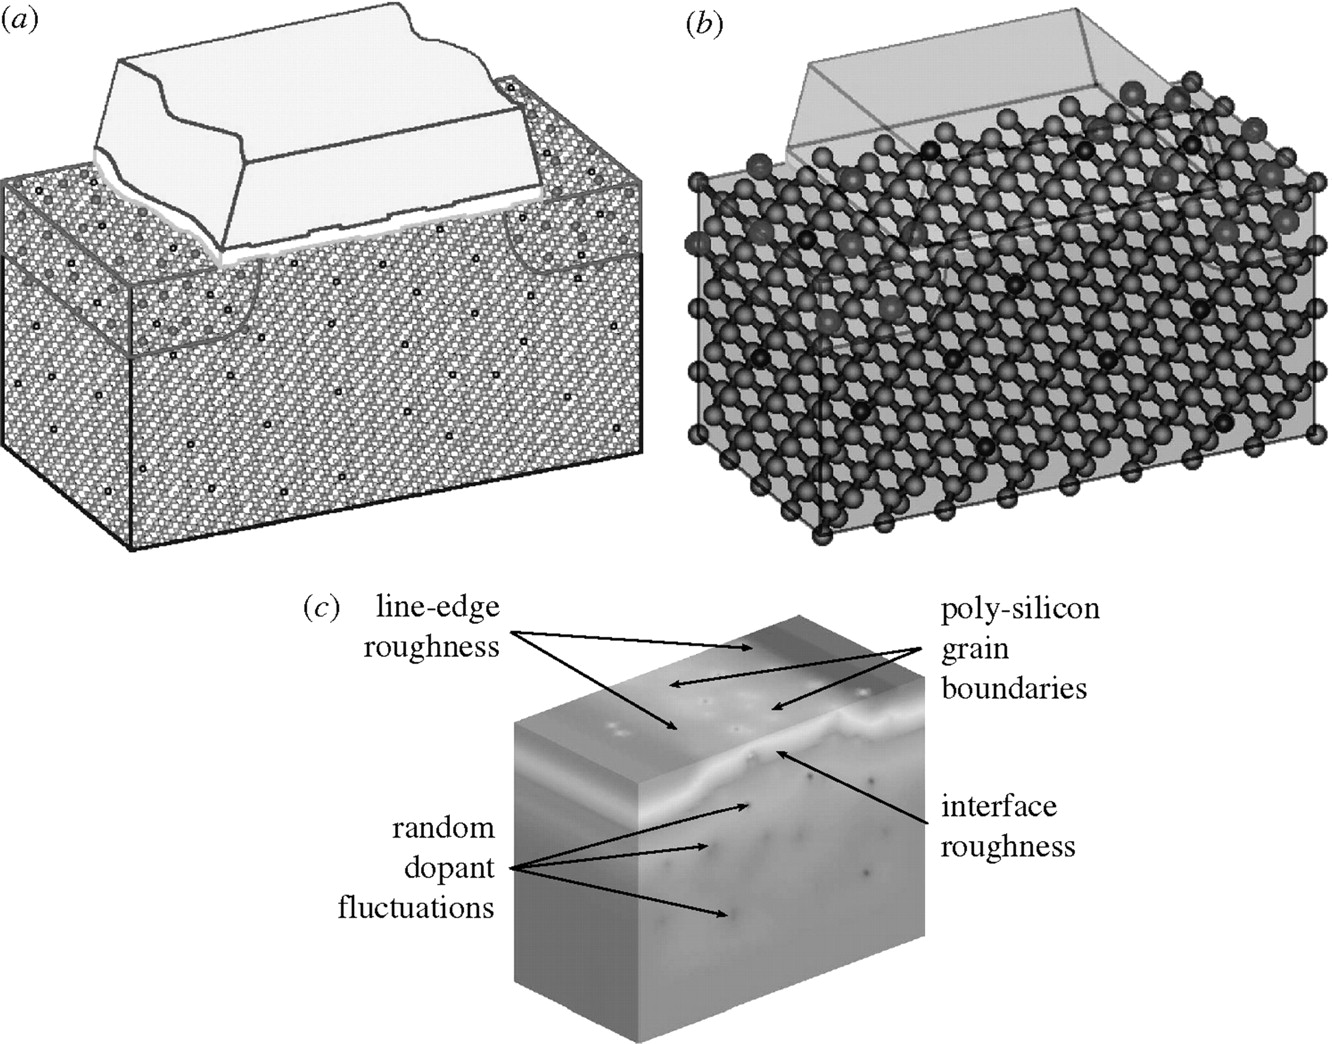
\includegraphics[width=.5\textwidth]{transistorVariability.jpg}
\caption{Transistor Variability}
\label{fig:Fig2}
\legend{Source: \cite{walker2010optimizing}}
\end{figure}

These three types of variabilities, in conjunction, may prevent circuits from meeting their performance and power goals. Table \ref{tab:02} demonstrates the design impact of performance and power due to different types of variability.

\begin{table}[H]
\centering
\caption{Design impact on performance and power due to different types of variability}
\label{tab:02}
\legend{Source: \cite{rahimi2016variability}}
\resizebox{\textwidth}{!}{%
\begin{tabular}{|l|c|c|c|c|}
\hline
Property & Ease of measuring & Variability & Effects of Variability & Effect of missing specification \\ \hline
Performance & Medium & Medium: up to 60\% & L, W, R, C, Vth, \(\mu\) & Slower product, yield, timing error \\ \hline
Leakage Power & Easy & Large: up to 148\% & L, Vth, \(\mu\), tox & Shorter battery life, yield , heat \\ \hline
Dynamic Power & Difficult & Workload dependent & C,  \(\alpha\) & Shorter battery life, heat \\ \hline
\end{tabular}%
}
\end{table}

This work evaluates the effects caused by the physical variability. In FinFET, the physical variations are responsible for deviations in the device work function (WF), gate length (L\textsc{g}), fin height (H\textsc{fin}), fin thickness (T\textsc{si}) and parasitic resistances. It is shown in \cite{meinhardt2014impact} that work 
function fluctuation (WFF) is the main cause of threshold voltage (V\textsc{th}) variations. Alongside, in \cite{wang2011statistical} is shown the high correlation between the variability in I\textsc{on} and I\textsc{off} currents and V\textsc{th} fluctuation in the presence of granularity of the metal gate. The main cause of WFF is due to its dependency over the orientation of its metal grains. In the real fabrication process, metal gate devices are generally produced using multiple types of metal with different work functions randomly aligned. In the ideal fabrication process, metal gate devices have the gates manufactured with uniformly aligned metal and then, they have very low WFF deviation \cite{zimpeck2016finfet}.

At circuit level there is multiple techniques to predict and prevent errors: Tuning CMOS knobs, circuit topology optimizations, self-timed circuits, temporal and logical error masking, relaxed retiming and graceful degradation, and inexact circuits. Although, there are few approaches to decrease the process variability at its core. It is due to the technology dependency present in this problem \cite{rahimi2016variability}.

It can be observed that many works try to indicate the most robust design for a given type of circuit. For example, in \cite{dokania2013investigation} twelve different Full Adder topologies are analyzed considering delay, power and Power-Delay-Product (PDP) variability. It is used a 16nm bulk CMOS technology node in SPICE simulations with Process, Voltage and Temperature (PVT) variability being considered and Monte Carlo simulations performed. The authors concluded that Cell A, CLRCL and Cell B full adders presented the best results for all three metrics (Delay, Power and PDP).

In \cite{ames2016investigating} the effects of PVT variability in different full adder designs are investigated. The simulations are performed in HSPICE with the bulk CMOS 32nm node technology. With TGA and TFA architectures showing acceptable behavior under PVT variability with the lowest power consumption sensibility amongst the tested full adders - 11x smaller in comparison with Complementary Pass Transistor Logic (CPL) Full Adder.

In \cite{islam2011design} various popular 1-bit digital summing circuits functionality and robustness are analyzed in light of PVT variations with the best full adder being simulated in CNFET technology for comparison with the bulk CMOS version. The simulations are carried at the 22nm bulk CMOS and CNFET technology node in HSPICE. Its results show that the TGA has the strongest PVT variability robustness and its CNFET version provides over 3x, 1.14x and 1.1x less propagation delay, power dissipation and energy delay product (EDP) variations, respectively. This work does not consider the total power consumption of each full adder separately.

Some articles analyze the adoption of new technologies: \cite{guduri2015design} proposes a hybrid of bulk CMOS and CNFET (Carbon Nanotube Field Effect Transistor) Full Adder at 16nm in deep subthreshold operation region for ultralow-power applications simulated in SPICE which showed some improvement over its bulk CMOS Full Adder counterpart achieving 5\% and 1\% improvement in power, power-delay and energy-delay products and their variability, respectively.  

In \cite{islam2011variability} a new subthreshold-FinFET (Fin Field-Effect Transistor) Full Adder is proposed and compared over multiple full adders showing huge metric improvements provided by the FinFET technology up to 2.22x improvement in power variability. It was simulated in 32nm predictive technology model on HSPICE. 

It is notable that none of these works consider a layout approach for its simulations and do not address any novel general technique which can be applied to a range of different types of circuits. Although, some works introduce novel designs.

\cite{federspiel201228nm} presents reliability comparison between 28nm bulk CMOS and FDSOI technologies at layout level, with FDSOI showing 32\% improved performance, 40\% reduced power consumption and improved matching, with its intrinsic reliability behavior similar to 28nm bulk at the device level. \cite{alioto2007delay} presents a study about the delay variability caused by supply variations in the Transmission Gate Full Adder (TGA). The experiments were performed at 90nm and 180nm bulk CMOS Technology in Spectre at layout level. It showed that lower supply voltages bring more delay variability to the circuit with the TG FA presenting worse results 15\% (25\%) for the 90 nm (180 nm) in comparison to static logic.

Some works focus on evaluating techniques: In \cite{zimpeck2016finfet} three dimensioning methods are applied on multiple circuits and their impact on variability robustness is analyzed. The simulations were performed considering a 14nm FinFET technology using HSPICE tool. The authors concluded that the Optimized Transistor Sizing (OTS) technique has the best ratio between nominal PDP and PDP under process variability.

\cite{ahmadi2017hybrid} introduces a new technique to improve the performance of digital circuits in the presence of variations. It consists of a hybrid of two former methods to prevent errors due to delay variations. The simulations were performed with a 45nm predictive technology using HSPICE and applied on ITC’99 and ISCAS’89 benchmarks circuits. The results show that this hybrid technique can tolerate process variations up to 27.3\% better than state-of-the-art techniques.

Among these works there is \cite{dokania2015circuit} on which a novel technique based on the replacement of Full Adder’s internal inverters with low voltage Schmitt Triggers for PVT variability robustness improvement is originally introduced and applied on seven different full adder designs. The simulations were performed using the 16nm bulk CMOS predictive technology model in SPICE. It presented significant variability improvement up to 4.8x in PDP. Although, the improvements occur at the cost of an increase in the area and power dissipation of each design.    

Schmitt triggers are commonly used as internal circuits on systems to provide enhanced noise tolerance and robustness against random variations in the input waveforms. On a typical input (non-Schmitt trigger), its binary value will switch at the same point on the rising and falling edges. With a slow rising edge, the input will change near the threshold point. When the switching occurs, it will require current from the supply source. With current being pushed from the supply, it can cause a voltage drop across the circuit causing a shift in the threshold voltage. 

If the threshold shifts, it will cross the input causing it to switch again. It can go indefinitely causing oscillation. The same thing can happen if there is noise on the input. Schmitt Triggers are applied in these cases to filter noise introducing superior and inferior threshold voltages, as shown in Figure \ref{fig:Fig3}.c. The difference between the thresholds is called Hysteresis \cite{WinNT}, its curve is shown at \ref{fig:Fig3}.a. According to the Schmitt Trigger behavior, it can mitigate the influence of variations in the inputs product of PVT variability. In figure \ref{fig:Fig3}.c is shown a classical CMOS Schmitt Trigger design. 

\begin{figure}[ht]
\centering
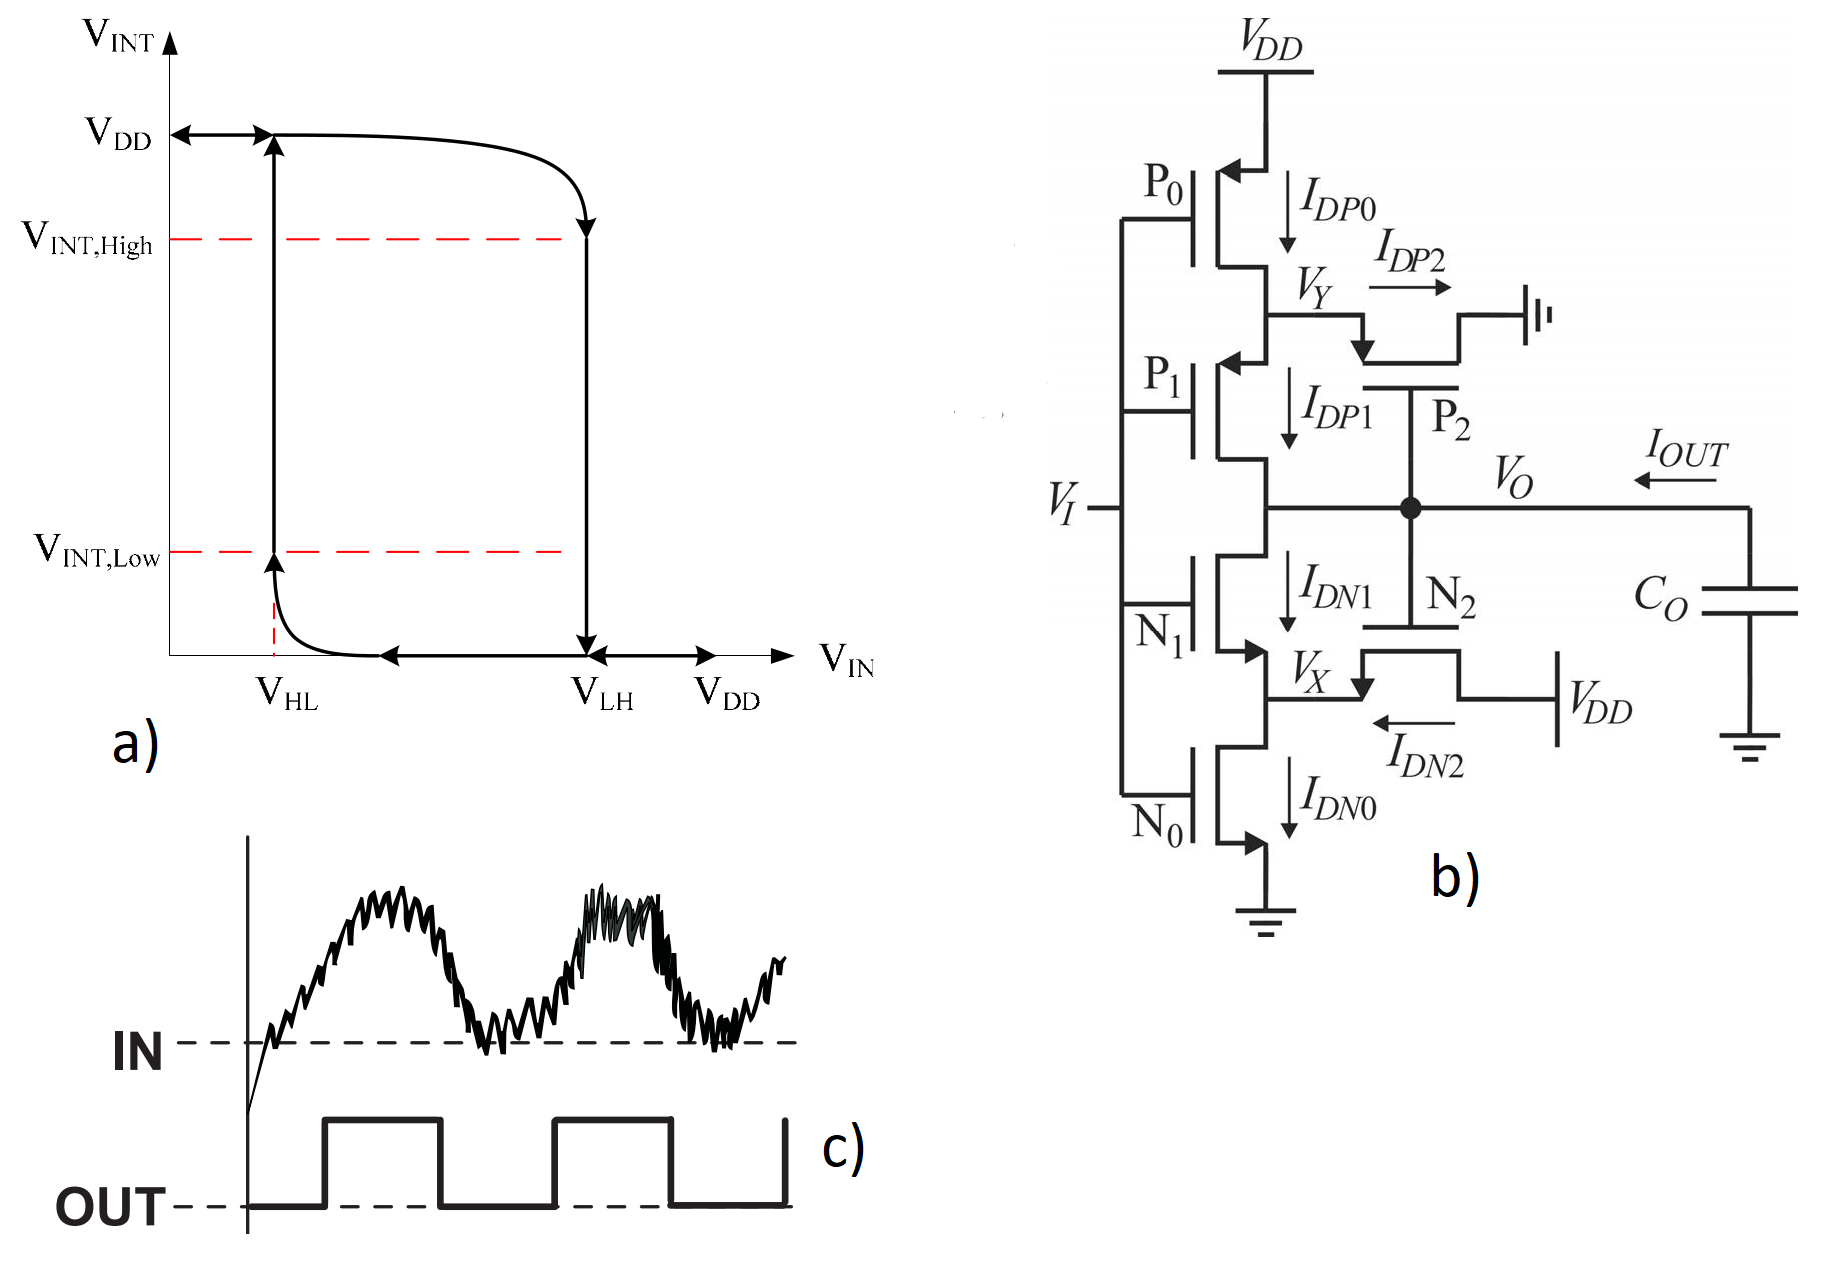
\includegraphics[width=1\textwidth]{Hysteresis.png}
\caption{a) General Schmitt Trigger's hysteresis curve b) Classical CMOS Schmitt Trigger Topology c) Typical signal filtering with Schmitt Trigger.}
\label{fig:Fig3}
\legend{Source: \cite{WinNT}}
\end{figure}

This technique is tested in several works: In \cite{ahmad2016single} it is presented a novel Schmitt-trigger-based single-ended 11T SRAM cell. It analyses its performance against seven different SRAM topologies. The novel cell showed the least energy consumption per operation with the smallest leakage power and a 6.9x higher Ion/Ioff ratio. Further PVT variability simulations confirmed the robustness of the design regarding read and write operation. The simulations were carried in 22nm predictive technology using HSPICE.

\cite{moghaddam2017design} presents a Schmitt trigger (ST) buffer using carbon nanotube FET (CNTFET). It was evaluated against other two buffers and showed, on average, 68\% higher critical charge and 53\% lower energy consumption and a huge gain considering PVT variability robustness. The simulations were carried in 16nm Stanford CNTFET model using HSPICE.
	
Alongside, in \cite{samuel2016} the ST technique is applied on four Full Adders. It presented promising results regarding the power deviation due to the process variability with a decrease up to 79\% with a drawback of a significant increase in average energy consumption. The simulations were performed with the 16nm technology predictive technology model in NGSPICE. 

\chapter{Methodology}

For the experiments, there will be considered four different types of Full Adders topologies to evaluate their robustness to process variability with their internal inverters replaced by Schmitt Triggers. The Full Adders listed below have been chosen due to their promising results in related works \cite{ames2016investigating} \cite{dokania2015circuit} \cite{dokania2013investigation}:

\begin{enumerate}
    \item Complementary MOSFET Adder (CMOS)
    \item Transmission Gate Adder (TGA)
    \item Transmission Function Adder (TFA)
    \item Hybrid Full Adder
\end{enumerate}

The CMOS Full Adder is considered the most traditional Full Adder topology containing 28 Transistors arranged in a pull-up and pull-down networks, which are logically complementary. It has a full voltage swing and buffered Sum and Cout signal and the advantages of good conductibility and robustness when working with novel technologies and low voltages. However, it has high capacitance because each input is connected to the gate of at least a PMOS and NMOS device additionally, it shows the impact of the pull-up network that makes the circuit slower due to the low mobility of its holes \cite{beckett2002fine} \cite{devadas2017design} \cite{islam2011design}. 

Transmission Gate Full Adder \cite{weste1985principles} contains 16 transistors, and is a high speed and low power design. However, shows low driving capability which may be unacceptable in some cases where there is a long chain of full adders due to the increase in delay \cite{islam2011design}. The Transmission Function Adder is based on transmission gates as well, containing 20 transistors, working satisfactorily with low voltages but losing performance when cascaded due to the lack of supply/ground contacts and, consequently, driving capability \cite{navi2009novel}. Both TFA and TGA generate the XOR function (H = A XOR B) followed by an inverter which produces the XNOR function (H’). H and H’ are used to control the transmission gates generating the Sum and Cout outputs. The inverter generates delay between H and H’, which will cause the transmission gates to behave as pass transistors, that may introduce glitches and consequently, increase the power consumption of these cells. Additionally, TGA contains three inverters, one more than TFA. The inverters switching introduce more short-circuit power \cite{shams2000novel}.

Inspired by CMOS and CPL Full Adders architectures, the Hybrid Full Adder \cite{navi2009novel} contains 26 transistors, with the main advantage of a high output signal and low power properties. Although, the design shows high input capacitance for specific input vectors. The Full Adder designs are shown in Figure \ref{fig:Fig5}.

\begin{figure}[ht]
\centering
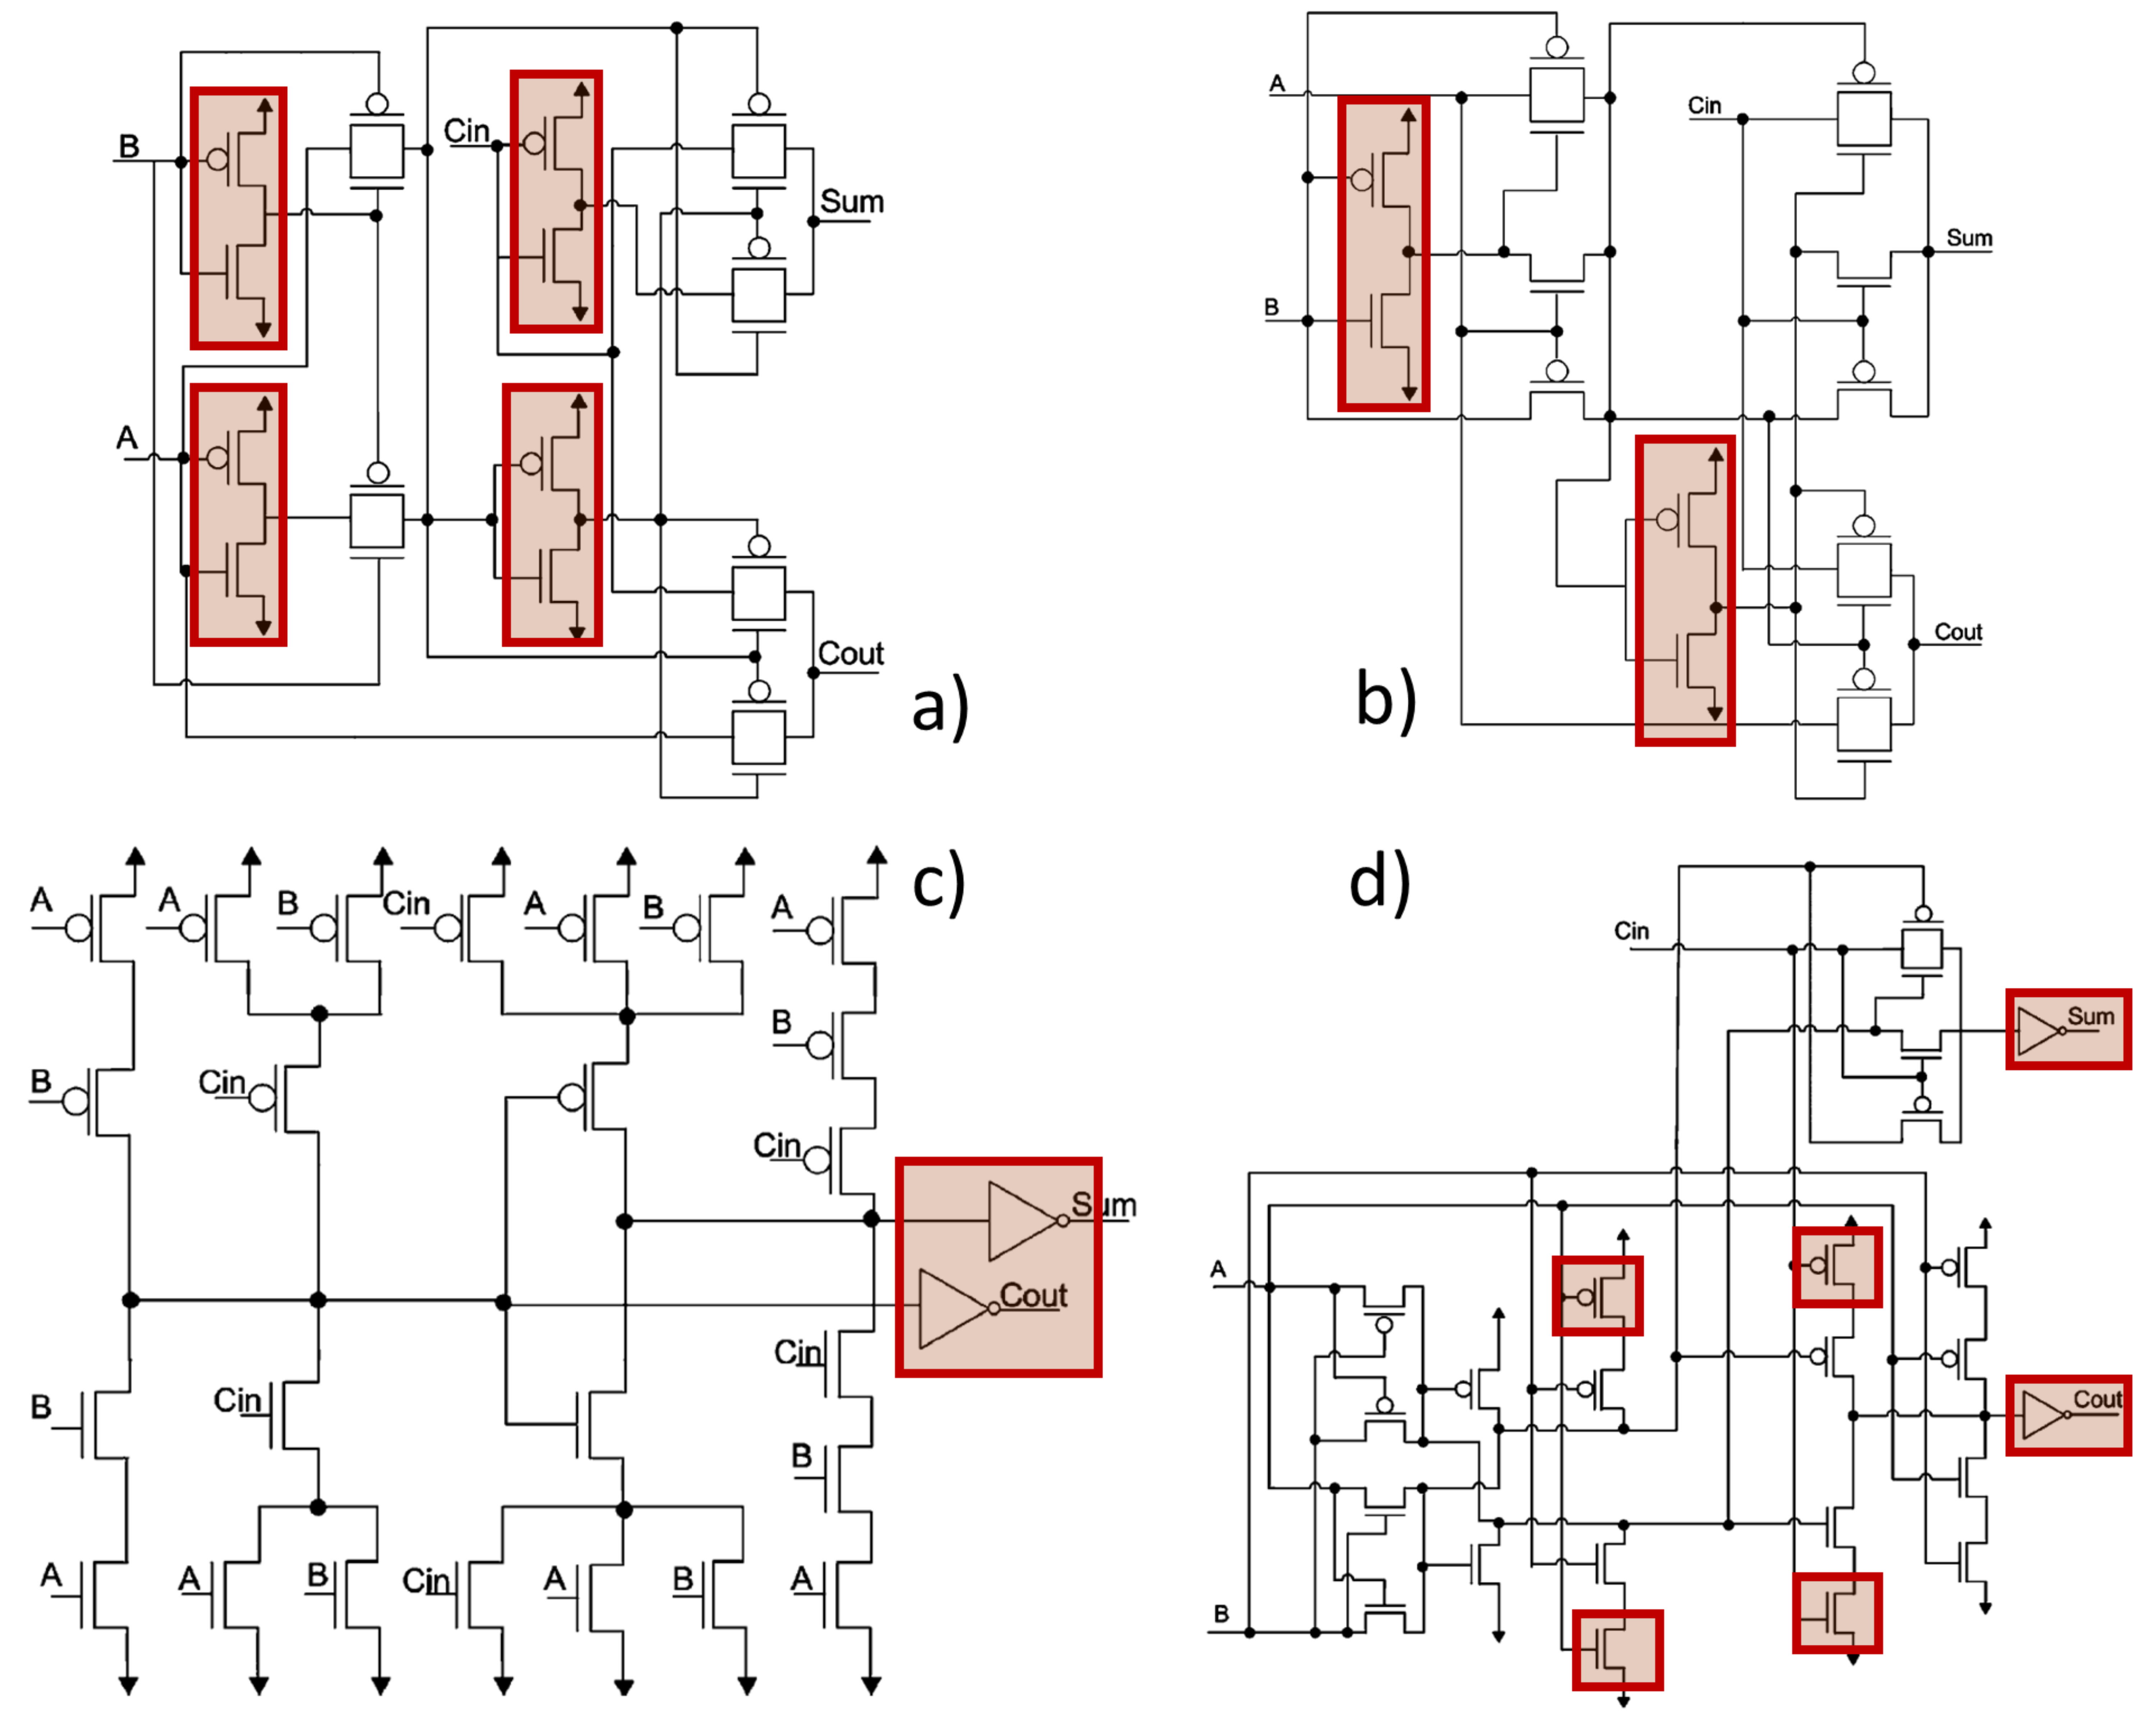
\includegraphics[width=1\textwidth]{FAs.png}
\caption{Full Adders with internal inverters to be replaced highlighted.}
\label{fig:Fig5}
\legend{Transmission Function Adder (a), Transmission Gate Adder (b), Mirror CMOS Adder (c) and Hybrid Full Adder (d).
Source: \cite{samuel2016}}
\end{figure}

A variety of CMOS Schmitt Trigger designs have been proposed and implemented over the years, with the conventional 6T-CMOS Schmitt Trigger proposed in \cite{doki1984cmos} exhibiting the wanted characteristics of different high-to-low and low-to-high transition threshold voltages, giving rise to hysteresis. The ST inverter circuit used in this work was inspired by \cite{zhang2003low} and modified in \cite{dokania2015circuit} to achieve the desired inverting characteristic, as shown in Figure \ref{fig:sub1}. It is designed for operation at a supply voltage of 0.4V in order to achieve low power consumption, and consists of the junction of two inverters where the output from the second one will be the bulk for the first one.  

In this design a dynamic body-bias technique is applied through a feedback mechanism to a standard CMOS inverter circuit, thus allowing a change in the threshold voltages of two MOSFETs, implying a change in the switching voltage. 

\begin{figure}[ht]
\centering
\begin{subfigure}{.5\textwidth}
  \centering
  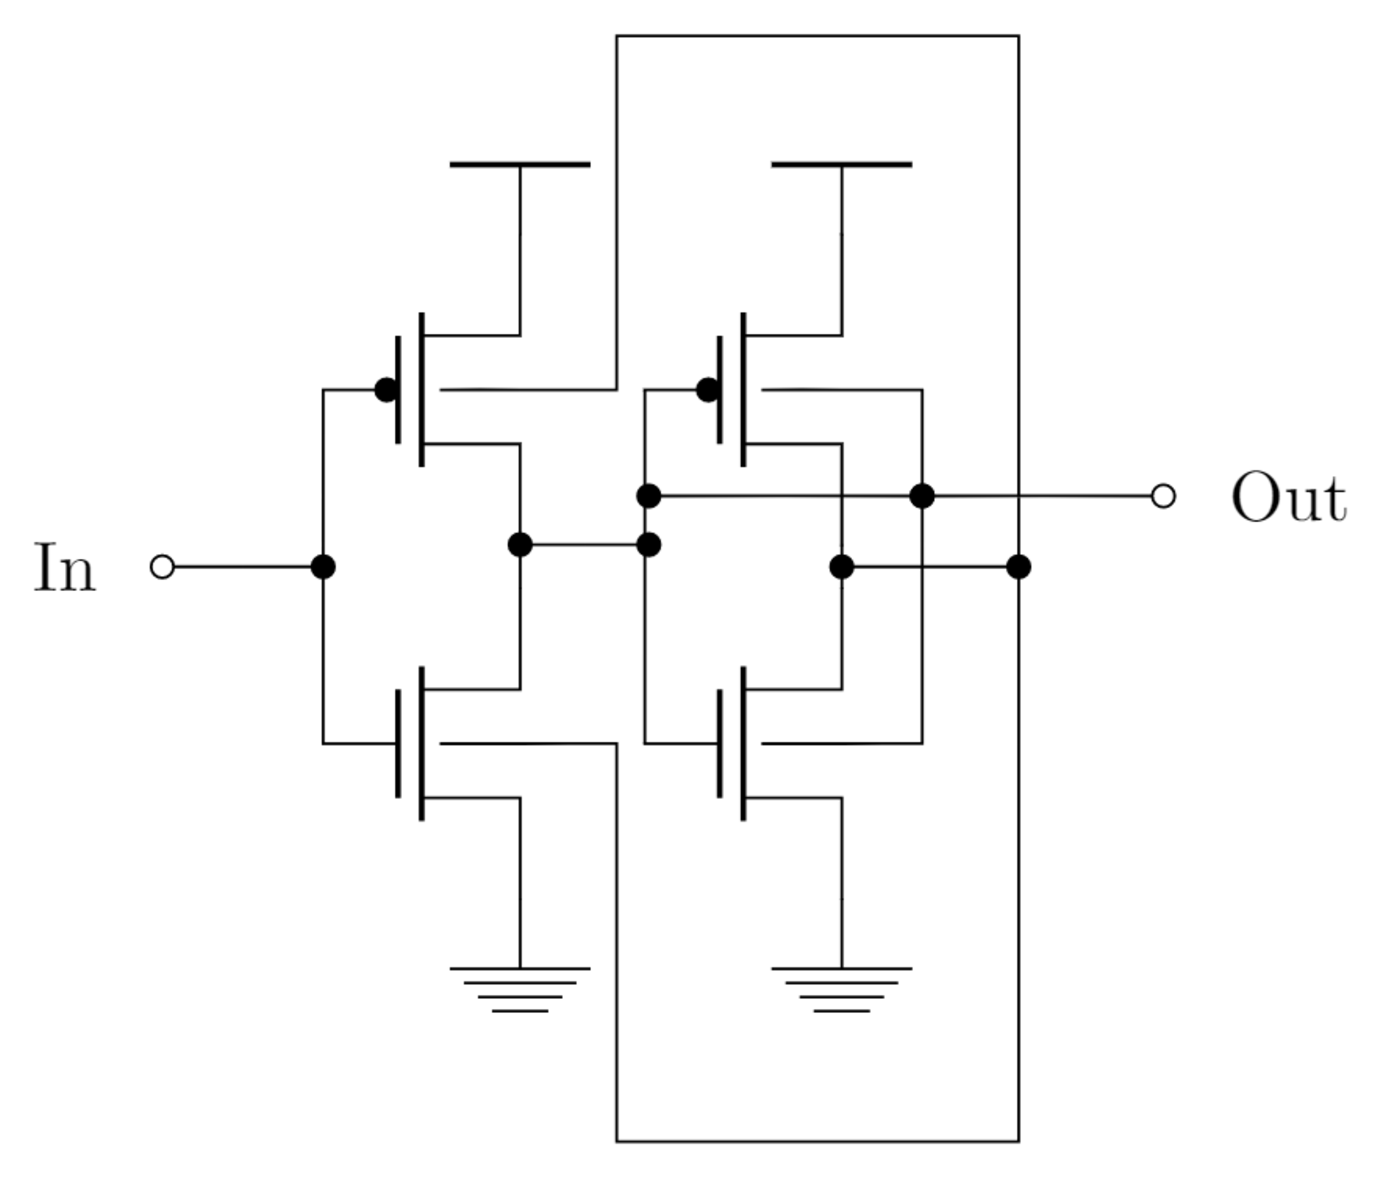
\includegraphics[width=.8\linewidth]{STOriginal.eps}
  \caption{ST Inverter applied on \citet{dokania2015circuit}}
  \label{fig:sub1}
\end{subfigure}%
\begin{subfigure}{.5\textwidth}
  \centering
  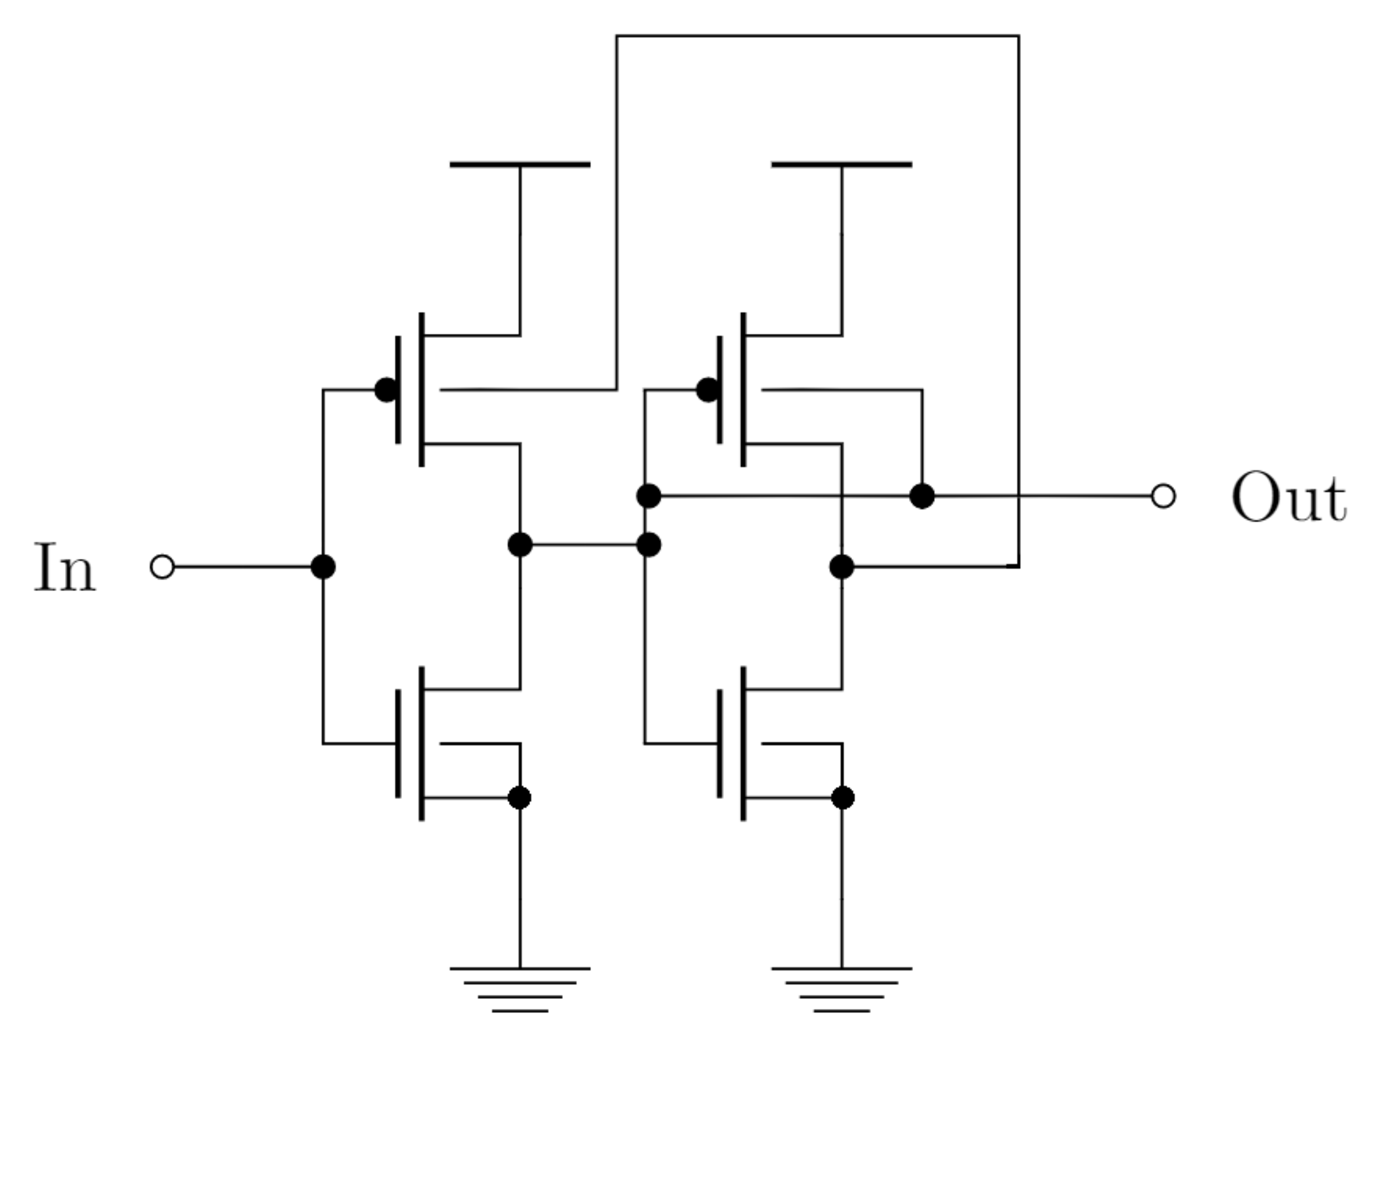
\includegraphics[width=.8\linewidth]{STcorrigido.eps}
  \caption{Modified ST Inverter applied in this work}
  \label{fig:sub2}
\end{subfigure}
\caption{Original and modified STs side-by-side}
\label{fig:test}
\end{figure}

\section{Layout Design}

All Full Adders layouts will be designed using the Virtuoso Electronic Design Automation (EDA) tool from Cadence\textregistered{} with the process design kit (PDK) of 7-nm FinFET (ASAP) from the Arizona State University in partnership with ARM \cite{clark2016asap7}. This PDK was chosen due to realistic design conjecture regarding the current design competencies. Due to limitations of ASAP7 technology, it is not possible to connect the NMOS bulks separately due to the shared substrate. Given that, the Schmitt Trigger behavior is preserved with only minor changes between charging and discharging delays due to the difference between PMOS and NMOS threshold voltages. The ST applied in this work is shown at Figure \ref{fig:sub2}.

The main PDK rules and lithography assumptions considered in this work are shown in Table \ref{layers}. To exemplify the PDK layers, the traditional CMOS Full Adder layout is shown in Fig. (FIGURA DO LAYOUT). For all layouts it was used a dense 7.5 M2 (Metal 2) track cell, baseline resulting in a 270nm cell height. This corresponds to three fins for each transistor. To make the bulk connections it is necessary a TAP-Cell. It is responsible to connect the NMOS and PMOS bulks to supply/ground, respectively, being possible to connect the PMOS bulks to another node. It is a technology restriction needed for the proper function of the circuit. Its layout has a length of 108nm resulting in an area of 0.02916 \(\mu\)m^{2}.

\begin{table}[]
\centering
\caption{Key layer lithography assumptions, widths and pitches}
\label{layers}
\begin{tabular}{|l|c|c|c|}
\hline
\multicolumn{1}{|c|}{\textbf{Layer}} & \textbf{Lithography} & \textbf{Width/drawn (nm)} & \textbf{Pitch (nm)} \\ \hline
\textbf{Fin}                         & SAQP                 & 6.5/7                     & 27                  \\ \hline
\textbf{Active (horizontal)}         & EUV                  & 54/16                     & 108                 \\ \hline
\textbf{Gate}                        & SADP                 & 21/20                     & 54                  \\ \hline
\textbf{SDT/LISD}                    & EUV                  & 25/24                     & 54                  \\ \hline
\textbf{LIG}                         & EUV                  & 16/16                     & 54                  \\ \hline
\textbf{VIA0-VIA3}                   & EUV                  & 18/18                     & 25                  \\ \hline
\textbf{M1-M3}                       & EUV                  & 18/18                     & 36                  \\ \hline
\end{tabular}
\end{table}

\section{Electrical Simulation}

The simulations were carried out in HSPICE considering the new netlist obtained after the physical verification flow and the parasitic capacitances extraction. Each full adder was designed with and without the Schmitt Triggers replacement to consider the penalties due to the adoption of the ST technique in terms of area, energy and performance.

The process variability evaluation was taken
through 2000 Monte Carlo (MC) simulations varying
the threshold voltage of the PMOS and NMOS devices
according to a Gaussian distribution considering a 3\(\sigma\) deviation and a 5\% variation on nominal values. For all experiments, it will be observed maximum values, mean (\(\mu\)), standard deviation (\(\sigma\)) and normalized standard deviation (\(\sigma\)/\(\mu\)) for each metric: delay, power and energy, where \(\sigma\)/\(\mu\) represents the sensibility of the cell to process variability. 

The reference values from ASAP7 technology for electrical simulations are shown in Table \ref{electPar}. To avoid underestimating effects of realistic input waveforms on design metrics, the simulations will be carried under a 5-bit ripple carry adder using copies of the 1-bit full adder cell with design metrics being calculated for the middle cell as shown in Figure \ref{fig:Fig6}. 

\begin{table}[H]
\centering
\caption{Parameters applied in the electrical simulations}
\label{electPar}
\begin{tabular}{|l|c|c|}
\hline
\textbf{Parameter}                                            & \multicolumn{2}{c|}{\textbf{7nm}}                                  \\ \hline
\textbf{Nominal Supply Voltage}                               & \multicolumn{2}{c|}{0.7 V}                                         \\ \hline
\textbf{Gate Length (L\textsc{g})}           & \multicolumn{2}{c|}{21nm}                                          \\ \hline
\textbf{Fin Width (W\textsc{fin})}              & \multicolumn{2}{c|}{6.5nm}                                         \\ \hline
\textbf{Fin Height (H\textsc{fin})}          & \multicolumn{2}{c|}{32nm}                                          \\ \hline
\textbf{Oxide Thickness (T\textsc{ox})}      & \multicolumn{2}{c|}{2.1nm}                                         \\ \hline
\textbf{Channel Doping}                                       & \multicolumn{2}{c|}{1x10^{22}m^{-3}}                                     \\ \hline
\textbf{Source/Drain Doping}                                  & \multicolumn{2}{c|}{2x10^{22}m^{-3}} \\ \hline
\multicolumn{1}{|c|}{\multirow{2}{*}{\textbf{Work Function}}} & NFET                            & 4.372                            \\ \cline{2-3} 
\multicolumn{1}{|c|}{}                                        & PFET                            & 4.8108                           \\ \hline
\end{tabular}
\end{table}

\begin{figure}[H]
\centering
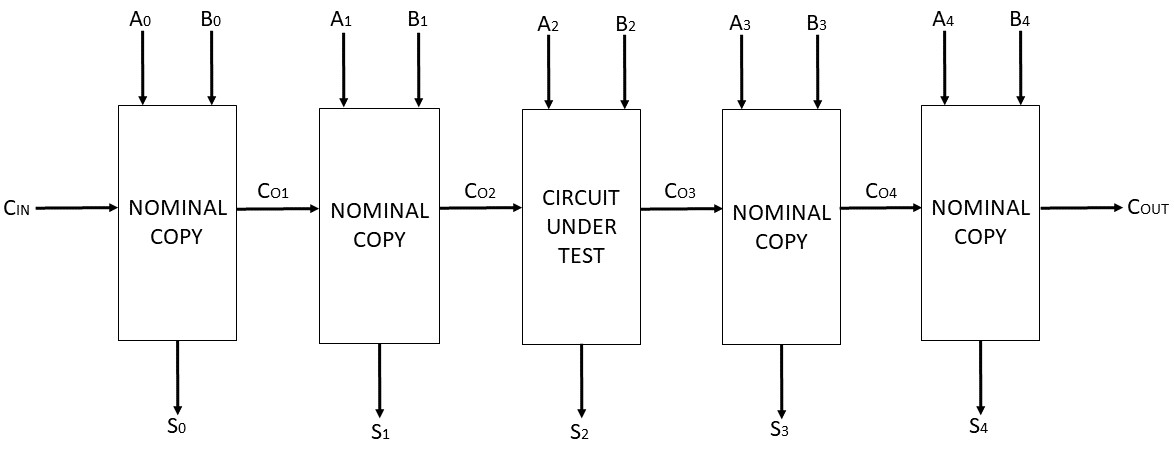
\includegraphics[width=.8\textwidth]{testbench.jpg}
\caption{Test Bench.}
\label{fig:Fig6}
\legend{Source: \cite{dokania2015circuit}}
\end{figure}



\chapter{Results}

The results will be shown in two parts for each Full Adder. The first part will concern the technique impact on nominal operation while the second part concerns for the near-threshold impact. Any improvement (worsening) of less than 5\% was disregarded in the analysis. 

\section{Mirror CMOS Full Adder}
At nominal level, the CMOS Full Adder has shown considerable improvement over energy variability robustness with 18.2\% (19\%) enhancement over Sum (Carry Out) output, showing no delay robustness improvements. At near-threshold level, there was a 18.7\% (11.6\%) and 20\% (12\%) delay and energy robustness improvements for the Sum (Carry Out) output. 

\section{Transmission Gate Full Adder}
At nominal level, the Transmission Gate Full Adder has shown an improvement of 15.77\% over Carry Out delays robustness while the Sum delay robustness worsened by 11.65\%. For energy robustness, only the Carry Out output showed improvements – over 31.32\%.
For the near-threshold level, there was an improvement of 31.53\% at Sum Output and a worsening of 19.14\% at Carry Out output. For energy there was huge improvements over 61.45\% (34\%) for the Sum (Carry Out) output.


\section{Transmission Function Full Adder}
At nominal level, the Transmission Function Full Adder showed an improvement over Sum delays robustness of 37.43\% and a worsening over Carry Out of 25.64\%. Although, on energy robustness it showed an improvement of 37.38\% (29.74\%) over the Sum (Carry Out) output. 
At near-threshold it showed a 64.74\% higher delay robustness at the Sum output, while at the Carry Out output it showed a 21.15\% lower robustness.  For energy robustness it showed great improvements with a 66.6\% (52.18\%) improvement concerning the Sum (Carry Out) output.


\section{Hybrid Full Adder}
For the Hybrid Full Adder, at nominal level, there was no improvements/worsening over the delay robustness. Although it showed considerable improvement on energy with 37.38\% (29.74\%) higher robustness for the Sum (Carry Out) output. 
At near-threshold there was improvement on all metrics with a 13.42\% (27.1\%) and 19.47\% (62\%) higher robustness on Sum and Carry Out delays (energy).

An improvement overview is shown in Figures \ref{fig:Fig41} and \ref{fig:Fig42} for nominal and near-threshold levels, respectively.

\begin{figure}[H]
\centering
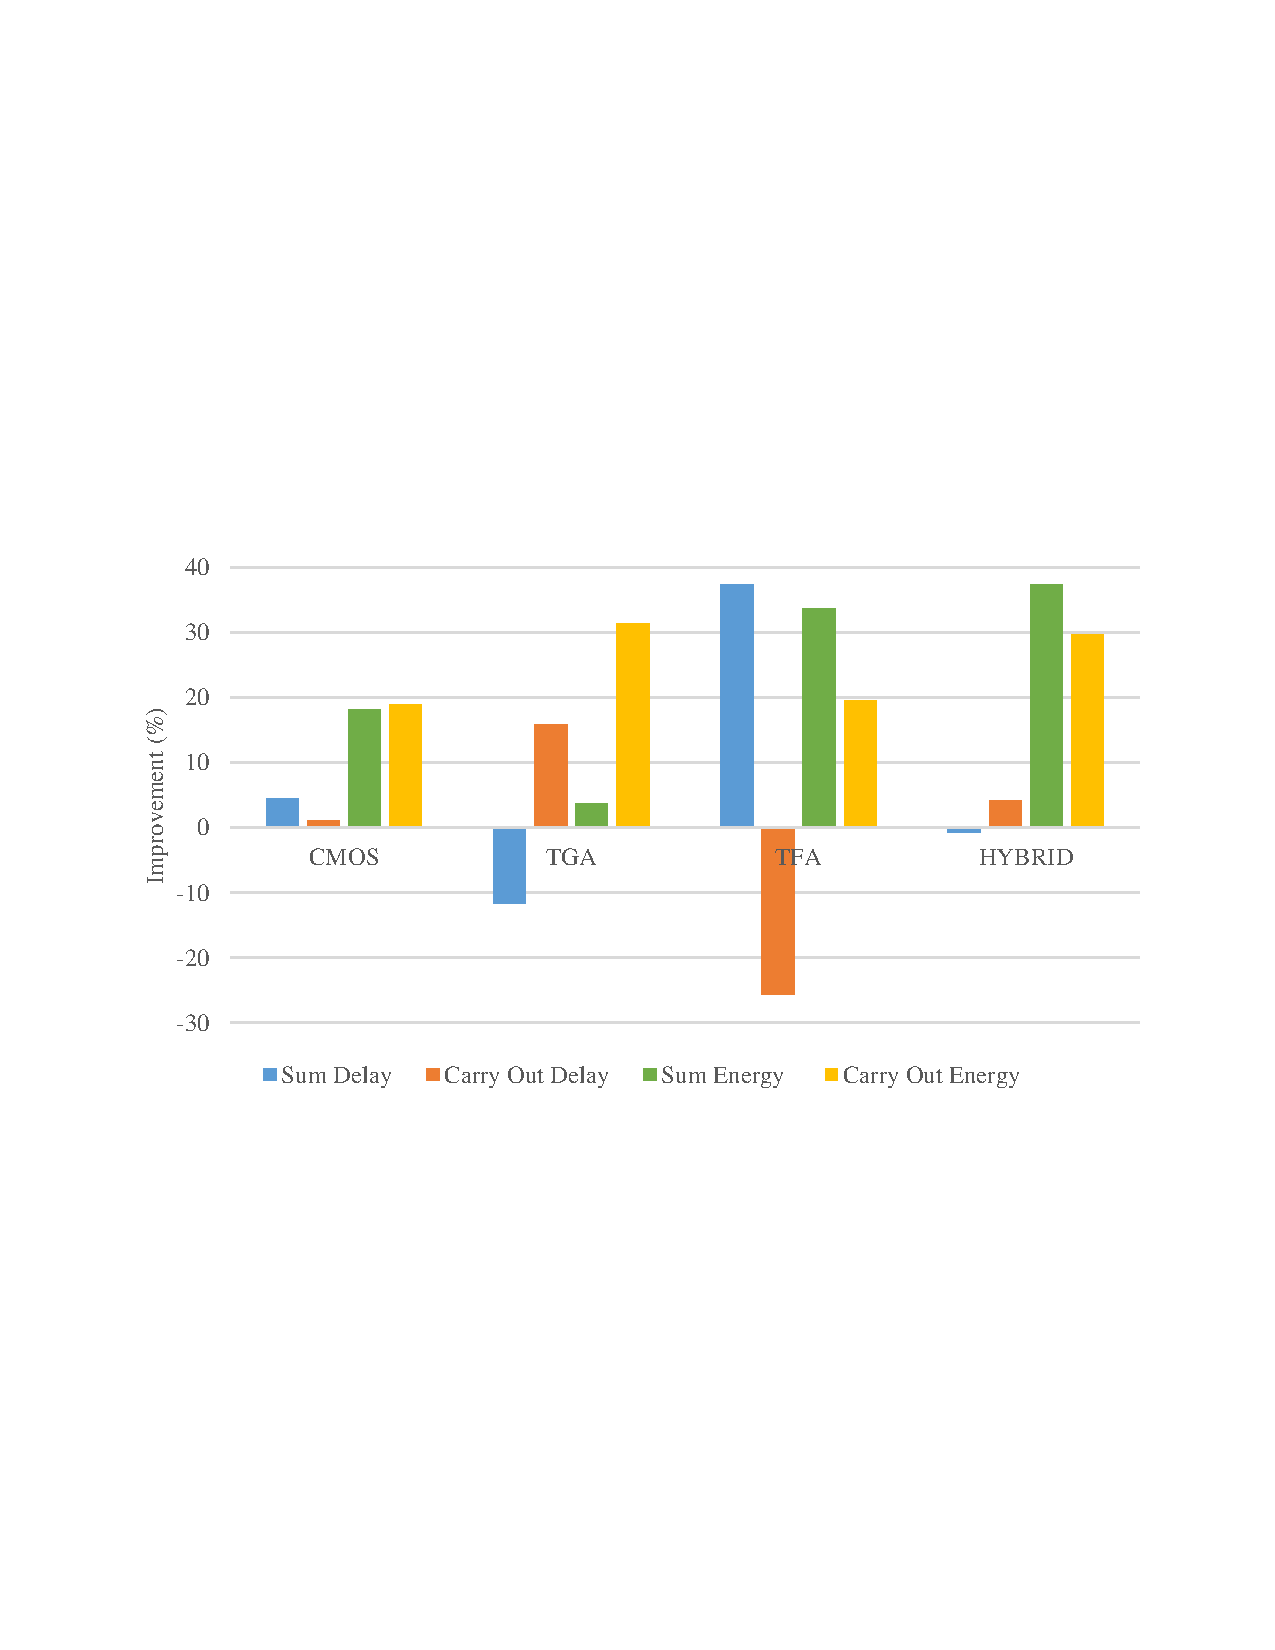
\includegraphics[width=\textwidth, trim={0 9.5cm 0 9cm},clip]{improvNominal.pdf}
\caption{Robustness improvements for each Full Adder at nominal operation.}
\label{fig:Fig41}
%\legend{Source: \cite{dokania2015circuit}}
\end{figure}

\begin{figure}[H]
\centering
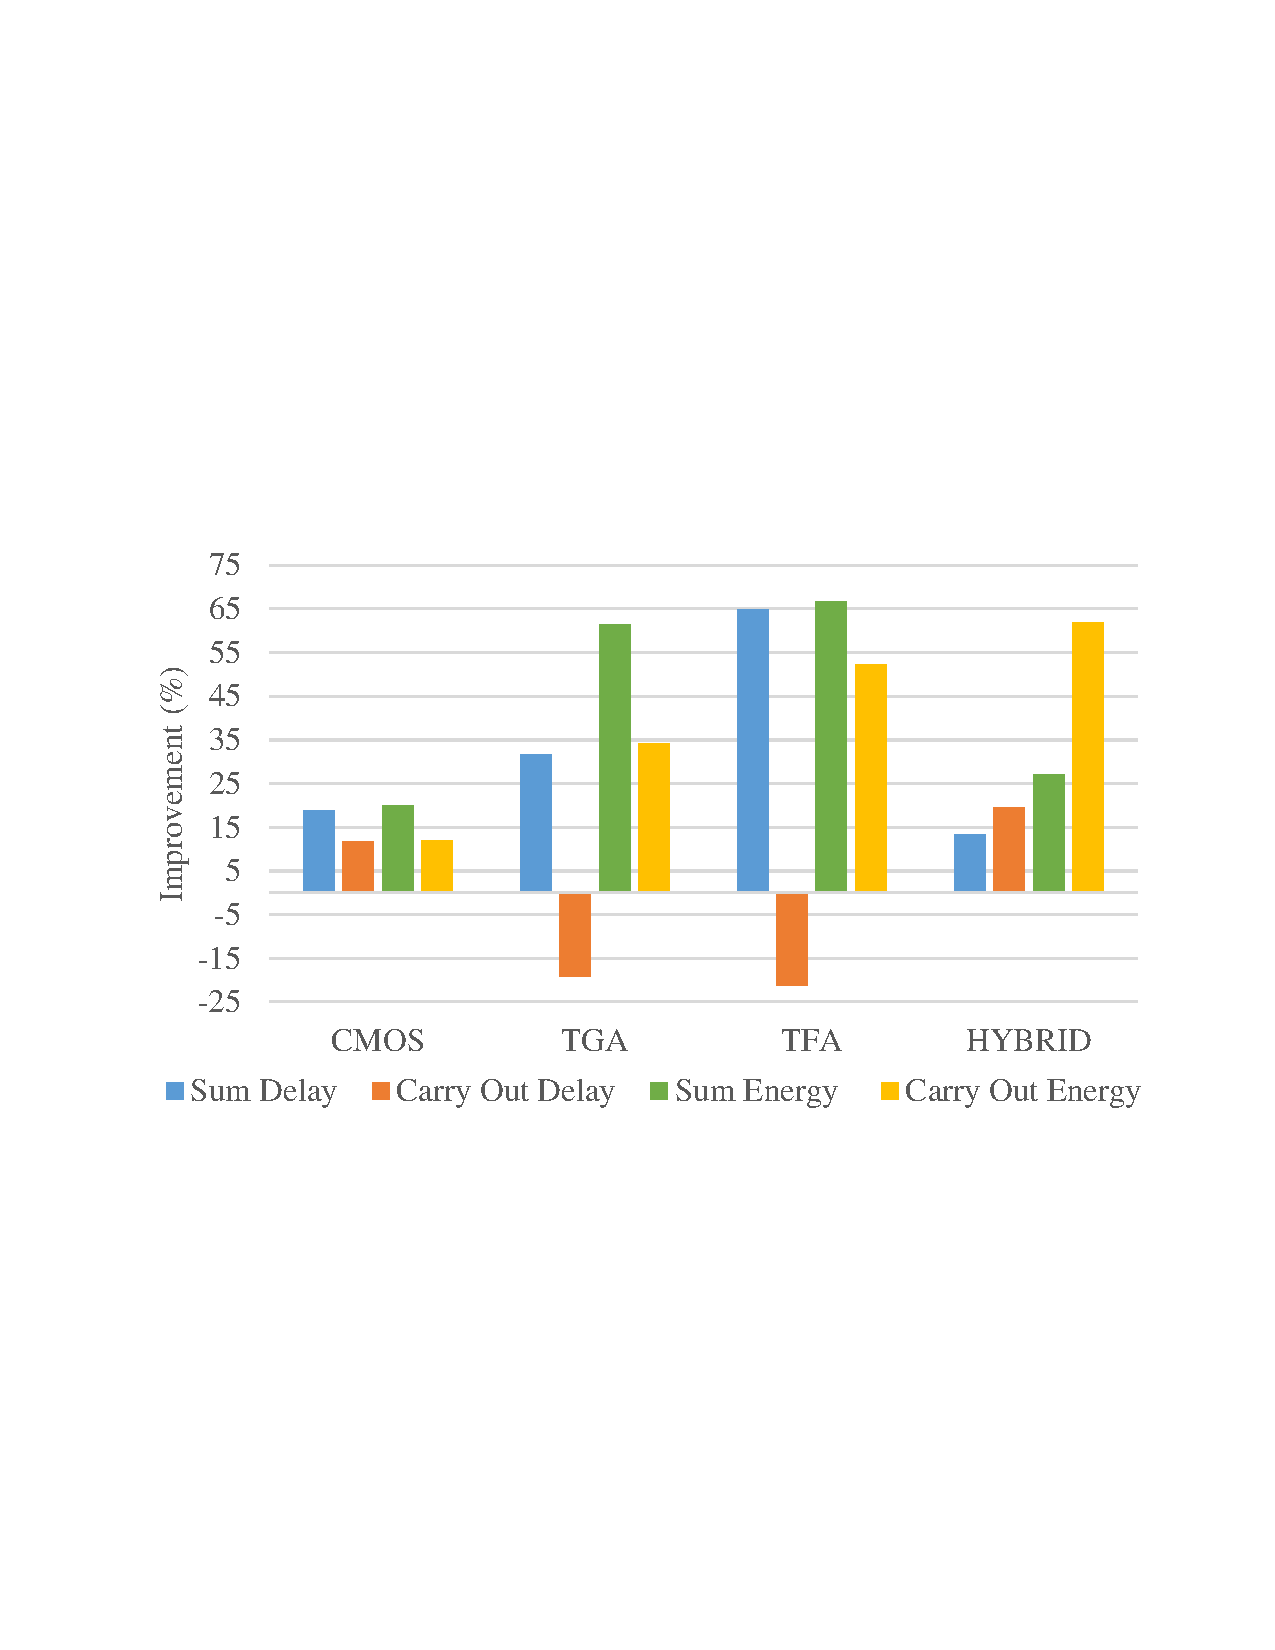
\includegraphics[width=\textwidth, trim={0 9.5cm 0 9cm},clip]{improvNT.pdf}
\caption{Robustness improvements for each Full Adder at near-threshold operation.}
\label{fig:Fig42}
%\legend{Source: \cite{dokania2015circuit}}
\end{figure}

\section{Discussion}
The technique presents considerable robustness improvements over all full adders. For nominal and near-threshold operation, the Hybrid and TFA (with Hybrid in second) adders showed the highest accumulated improvements, respectively.

Results make clear the advantage of the technique when considering energy variability robustness. Even when there was a worsening on delay robustness, the energy robustness presented improvements. The technique can introduce more delay variability given that variability determines the ST behavior as well, influencing its delays, which stacks with the impact of multiple transistors. In most cases there is either low variability and the technique’s inherently higher absolute deviation will cause a worsening in robustness or there is already some signal degradation due to the circuit’s area with the technique appliance only making it worse. 

The energy robustness is improved since the signals are restored for every simulation softening the stacked impact of the critical path’s transistors. Considering absolute metrics, the TFA showed the highest performance and lowest energy consumption for nominal operation. Although, with non-acceptable maximum values and absolute deviation. Which indicates heavy signal degradation, leaving the TFA for high-performance applications with little variability impact to deal with. The CMOS adder showed the lowest standard deviations being the most recommended for technology nodes with high variability. 

At near-threshold level, TFA and TGA showed the highest deviations and unacceptable maximum delays, which is expected due to their pass-transistor logic and inherent signal degradation. The Hybrid adder showed higher deviations, delays and similar energy consumption in comparison to the CMOS Adder. Given that, the CMOS adder remains as a considerable good choice for low power applications.

All absolute values for metrics are shown at Tables/Figures X, Y, Z.

\begin{figure}[H]
\centering
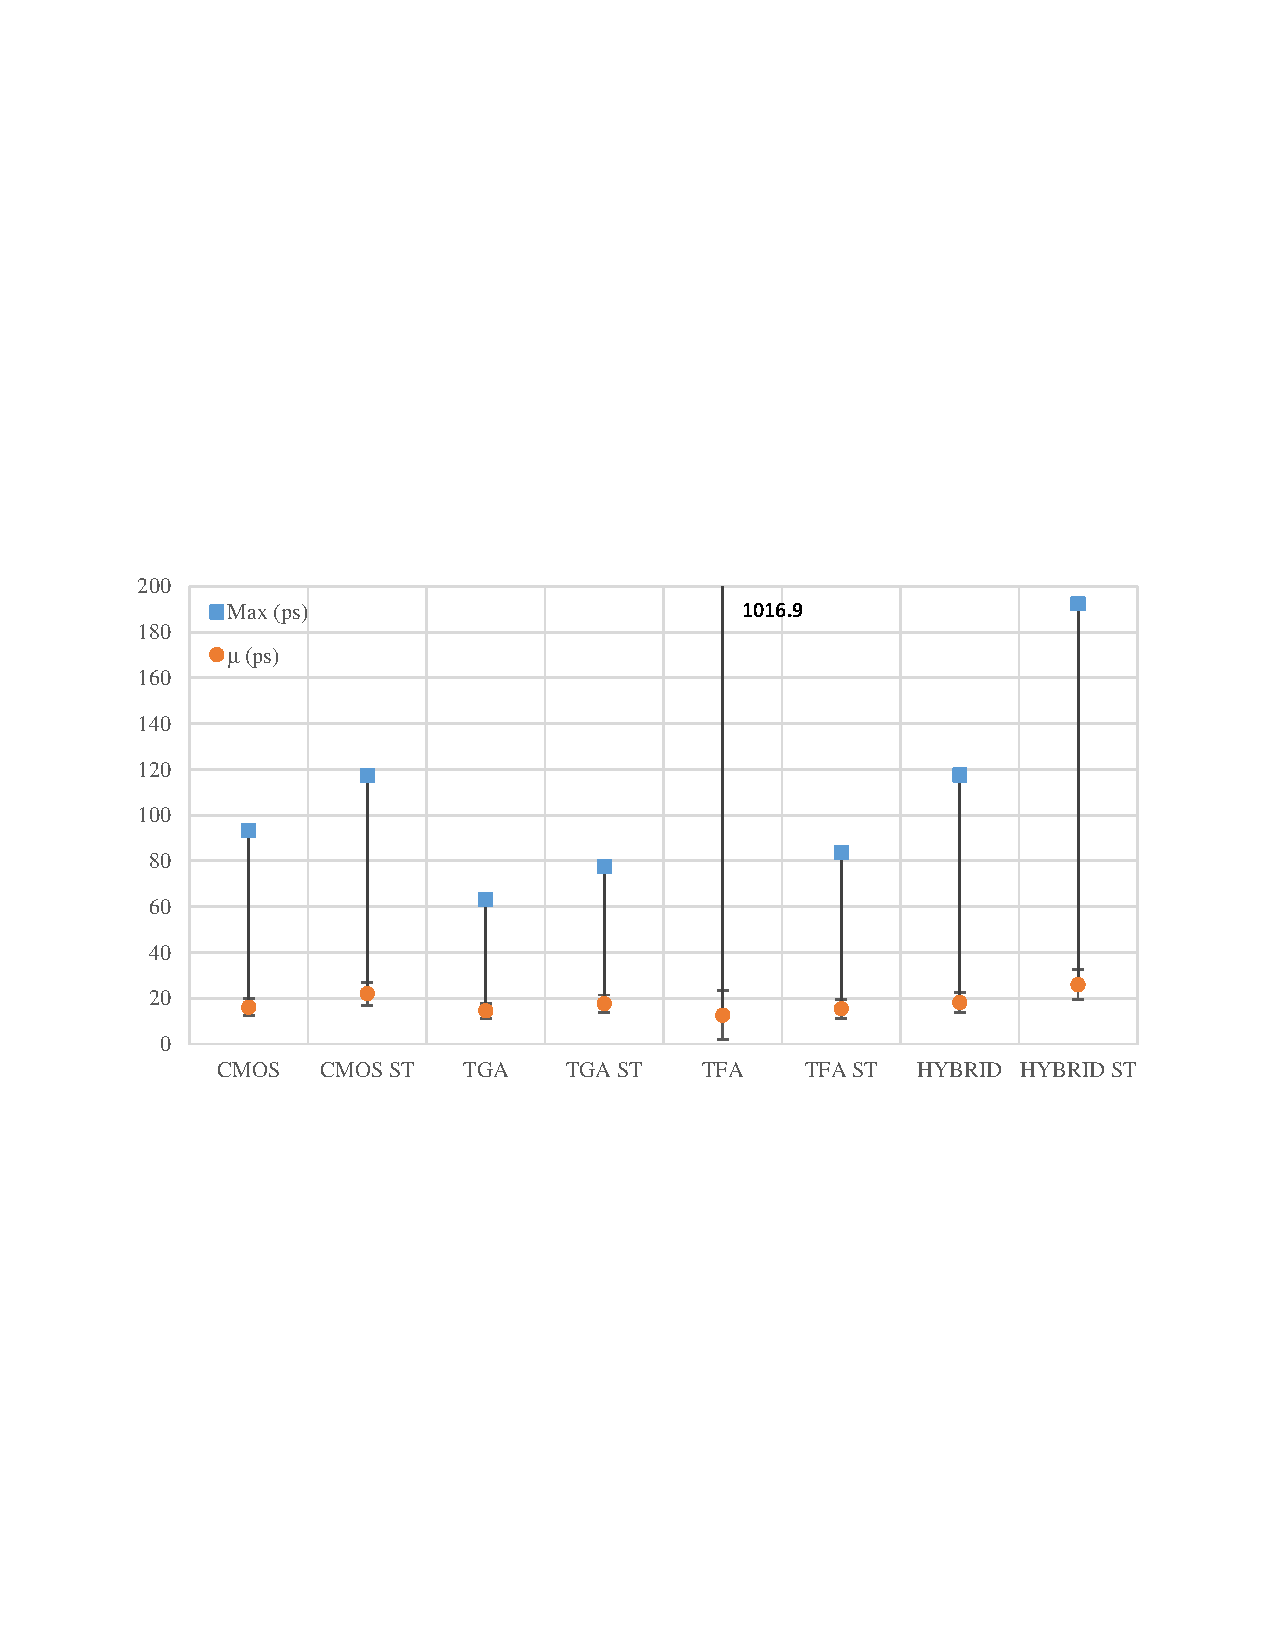
\includegraphics[width=\textwidth, trim={0 9.5cm 0 9cm},clip]{delaysNominalSum.pdf}
\caption{Propagation times for Sum output at nominal operation.}
\label{fig:Fig43}
%\legend{Source: \cite{dokania2015circuit}}
\end{figure}

\begin{figure}[H]
\centering
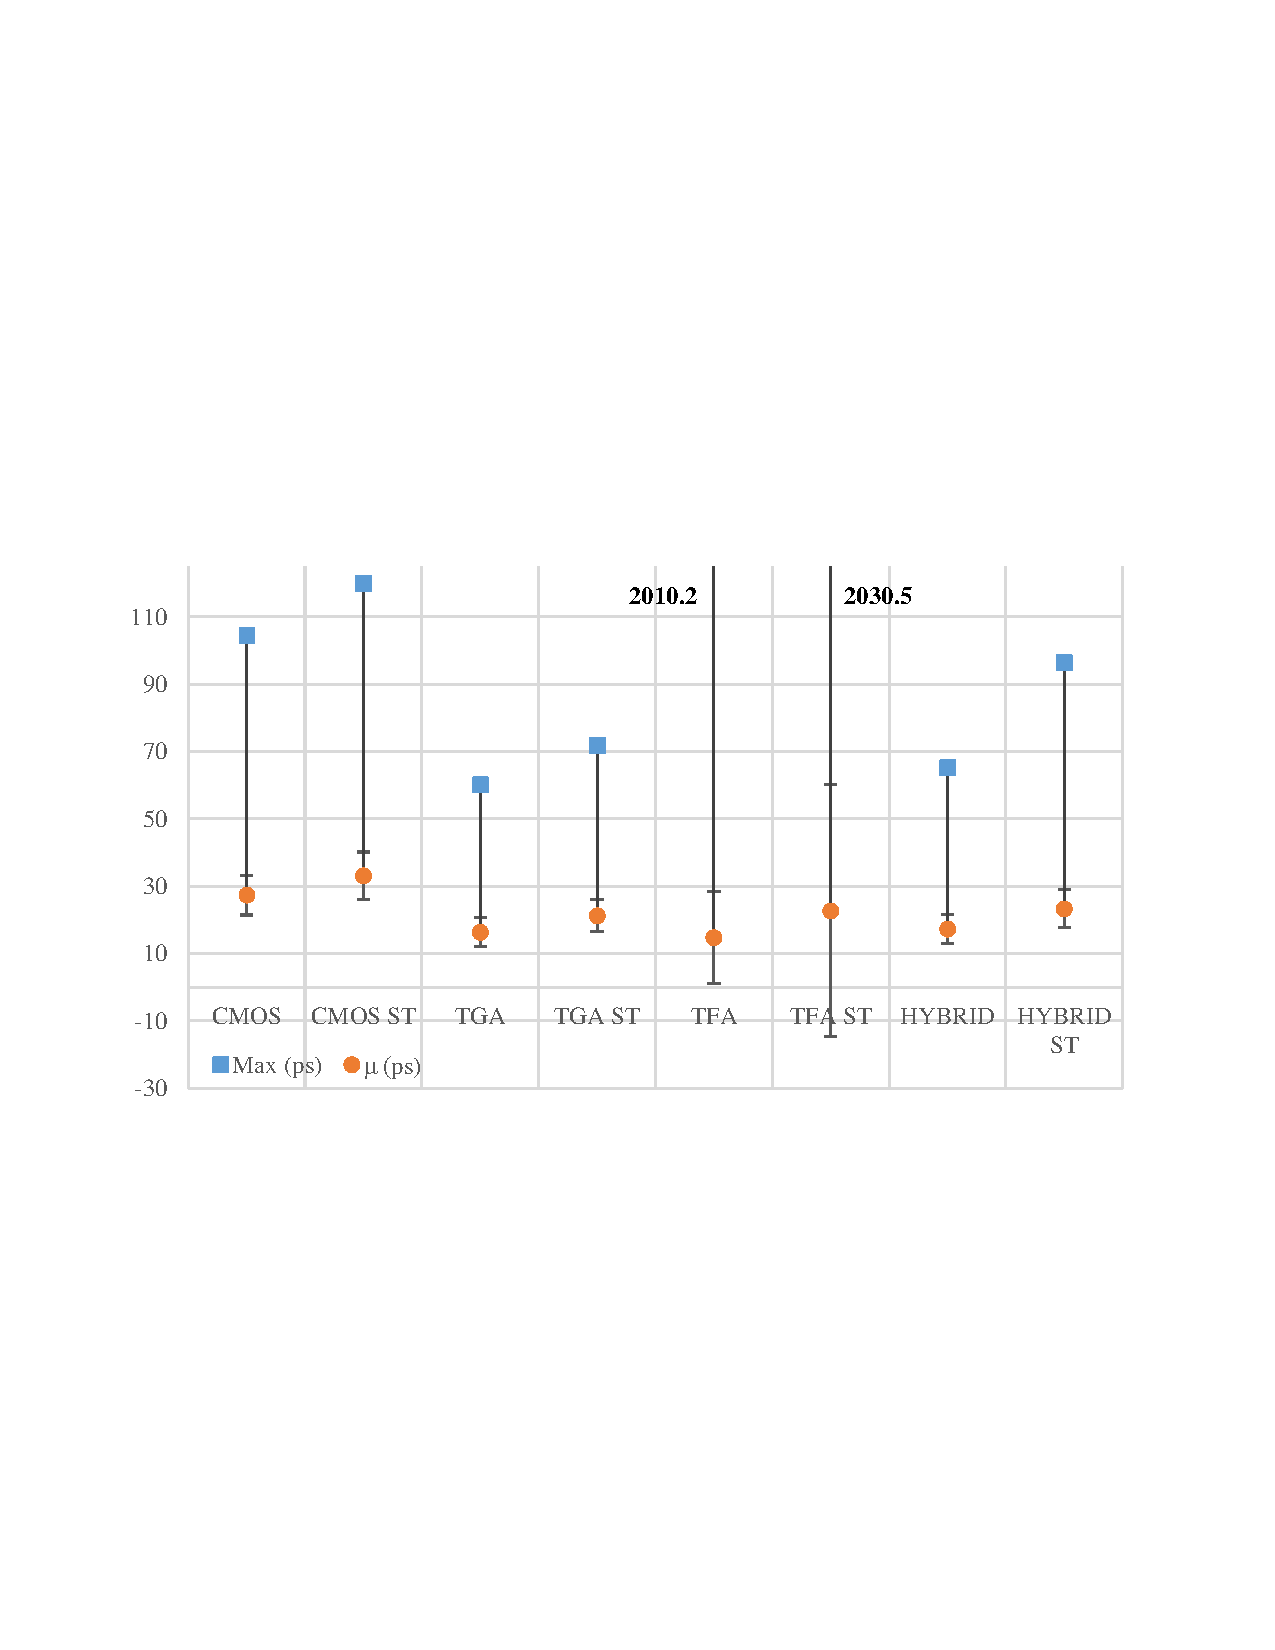
\includegraphics[width=\textwidth, trim={0 9cm 0 9cm},clip]{delaysNominalCarryOut.pdf}
\caption{Propagation times for Carry Out output at nominal operation.}
\label{fig:Fig44}
%\legend{Source: \cite{dokania2015circuit}}
\end{figure}

\begin{figure}[H]
\centering
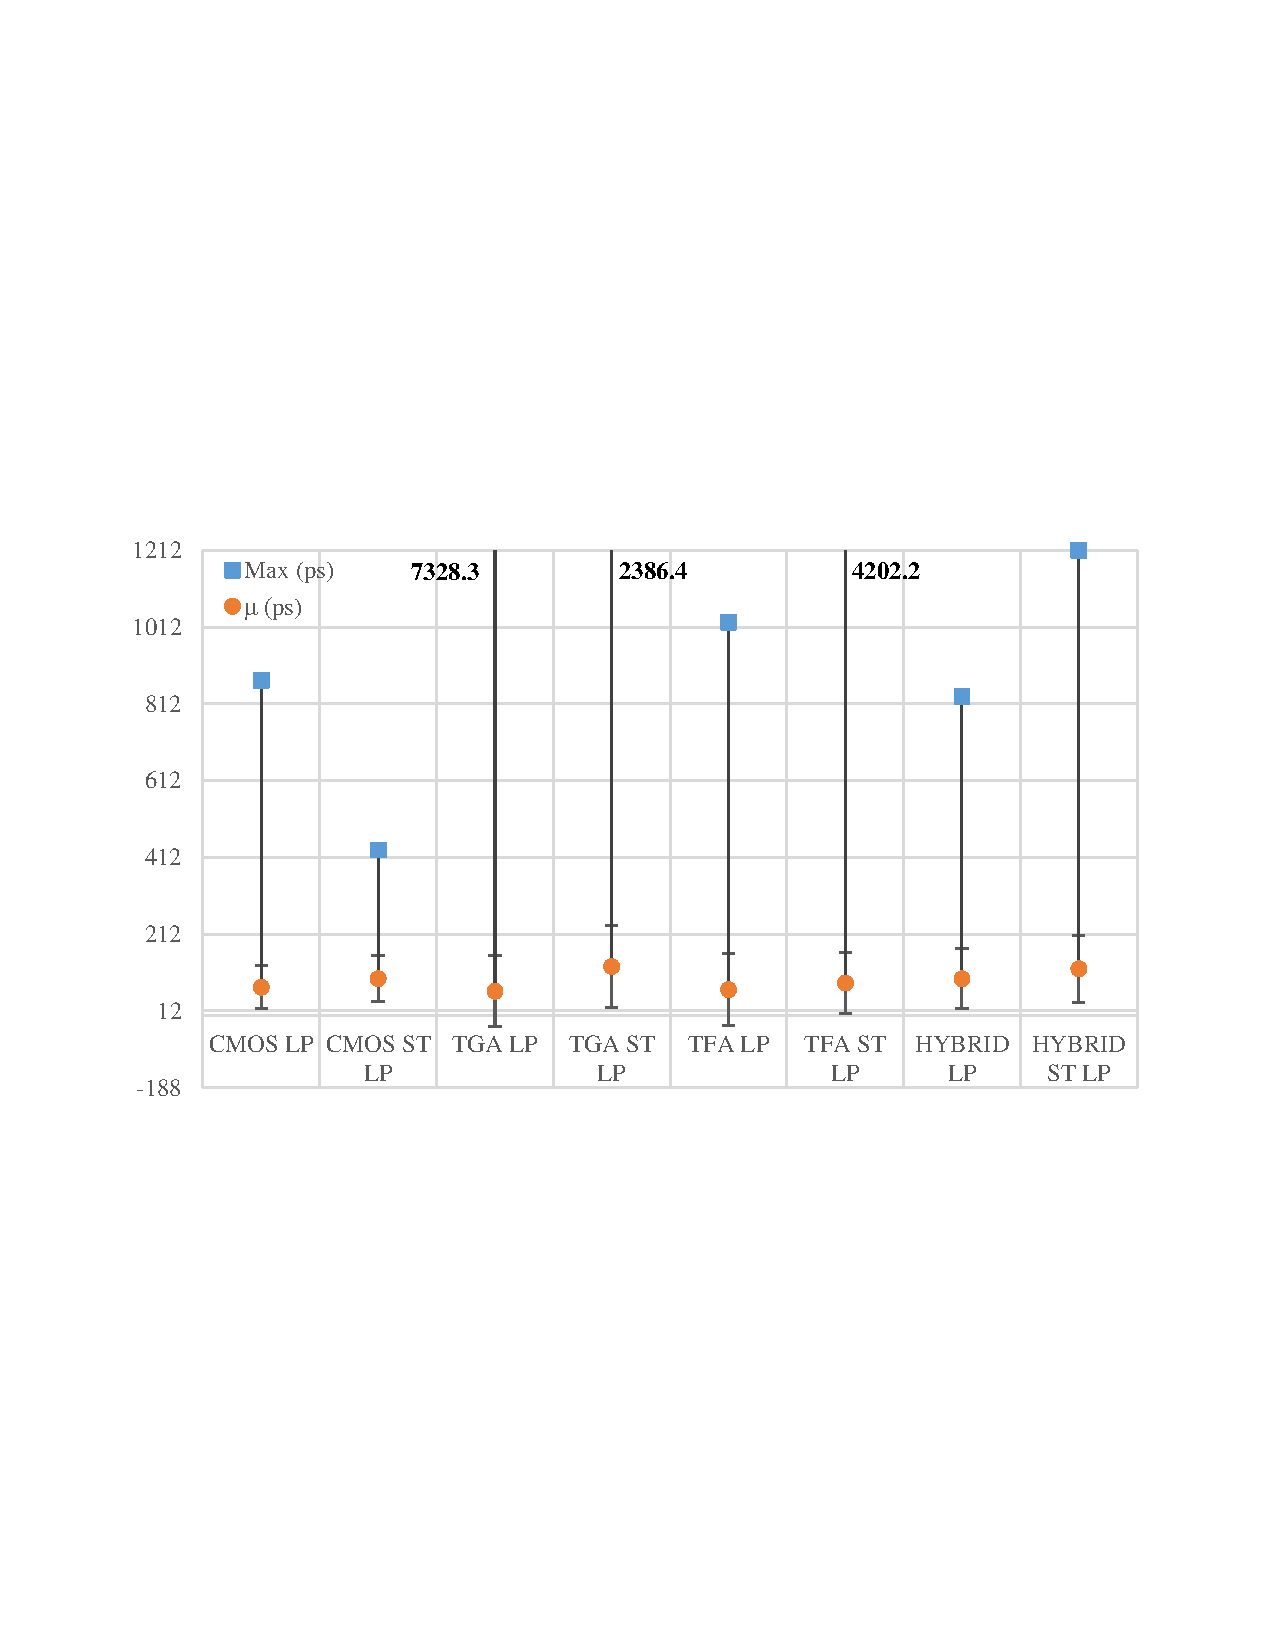
\includegraphics[width=\textwidth, trim={0 9cm 0 9cm},clip]{delaysNTSum.pdf}
\caption{Propagation times for Sum output at near-threshold operation.}
\label{fig:Fig45}
%\legend{Source: \cite{dokania2015circuit}}
\end{figure}

\begin{figure}[H]
\centering
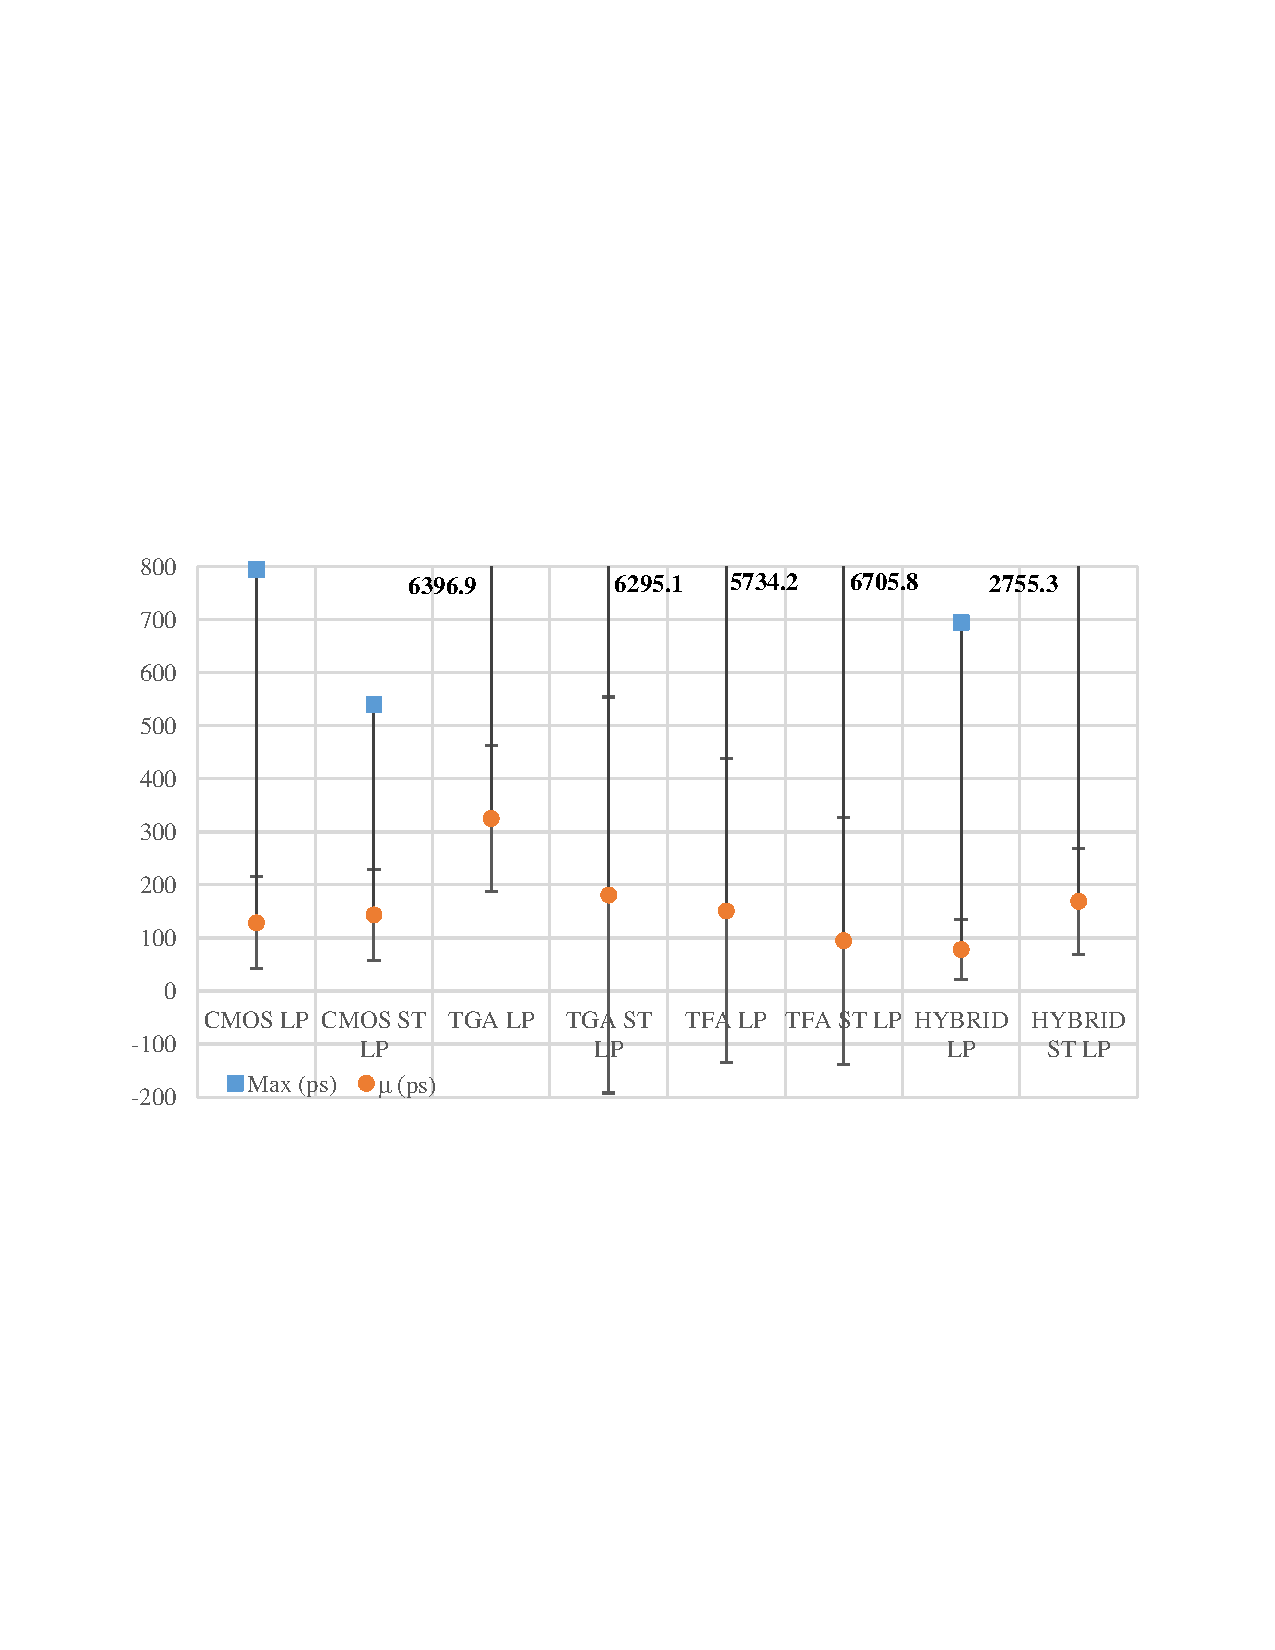
\includegraphics[width=\textwidth, trim={0 9cm 0 9cm},clip]{delaysNTCarryOut.pdf}
\caption{Propagation times for Carry Out output at near-threshold operation.}
\label{fig:Fig46}
%\legend{Source: \cite{dokania2015circuit}}
\end{figure}

\begin{figure}[H]
\centering
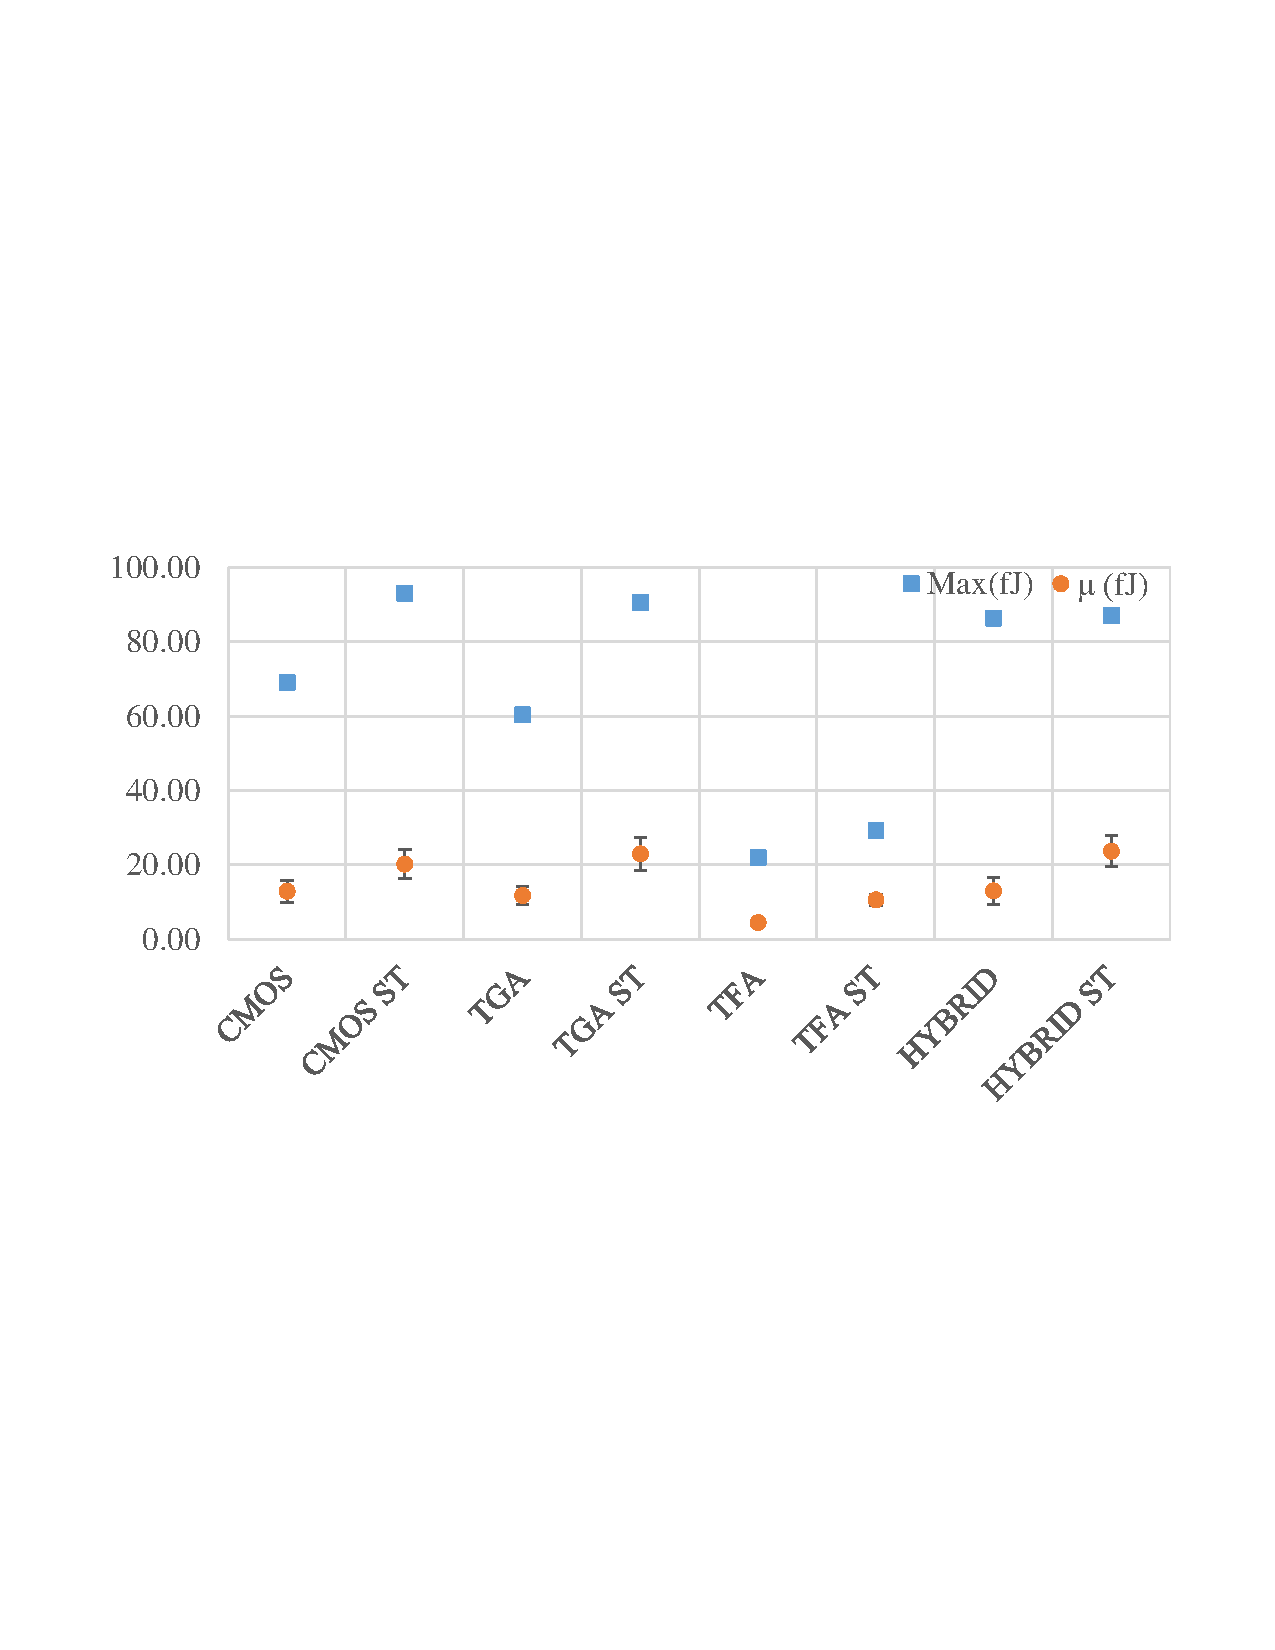
\includegraphics[width=\textwidth, trim={0 9cm 0 9cm},clip]{energyNominalSum.pdf}
\caption{Energy measures for Sum output at nominal operation.}
\label{fig:Fig47}
%\legend{Source: \cite{dokania2015circuit}}
\end{figure}

\begin{figure}[H]
\centering
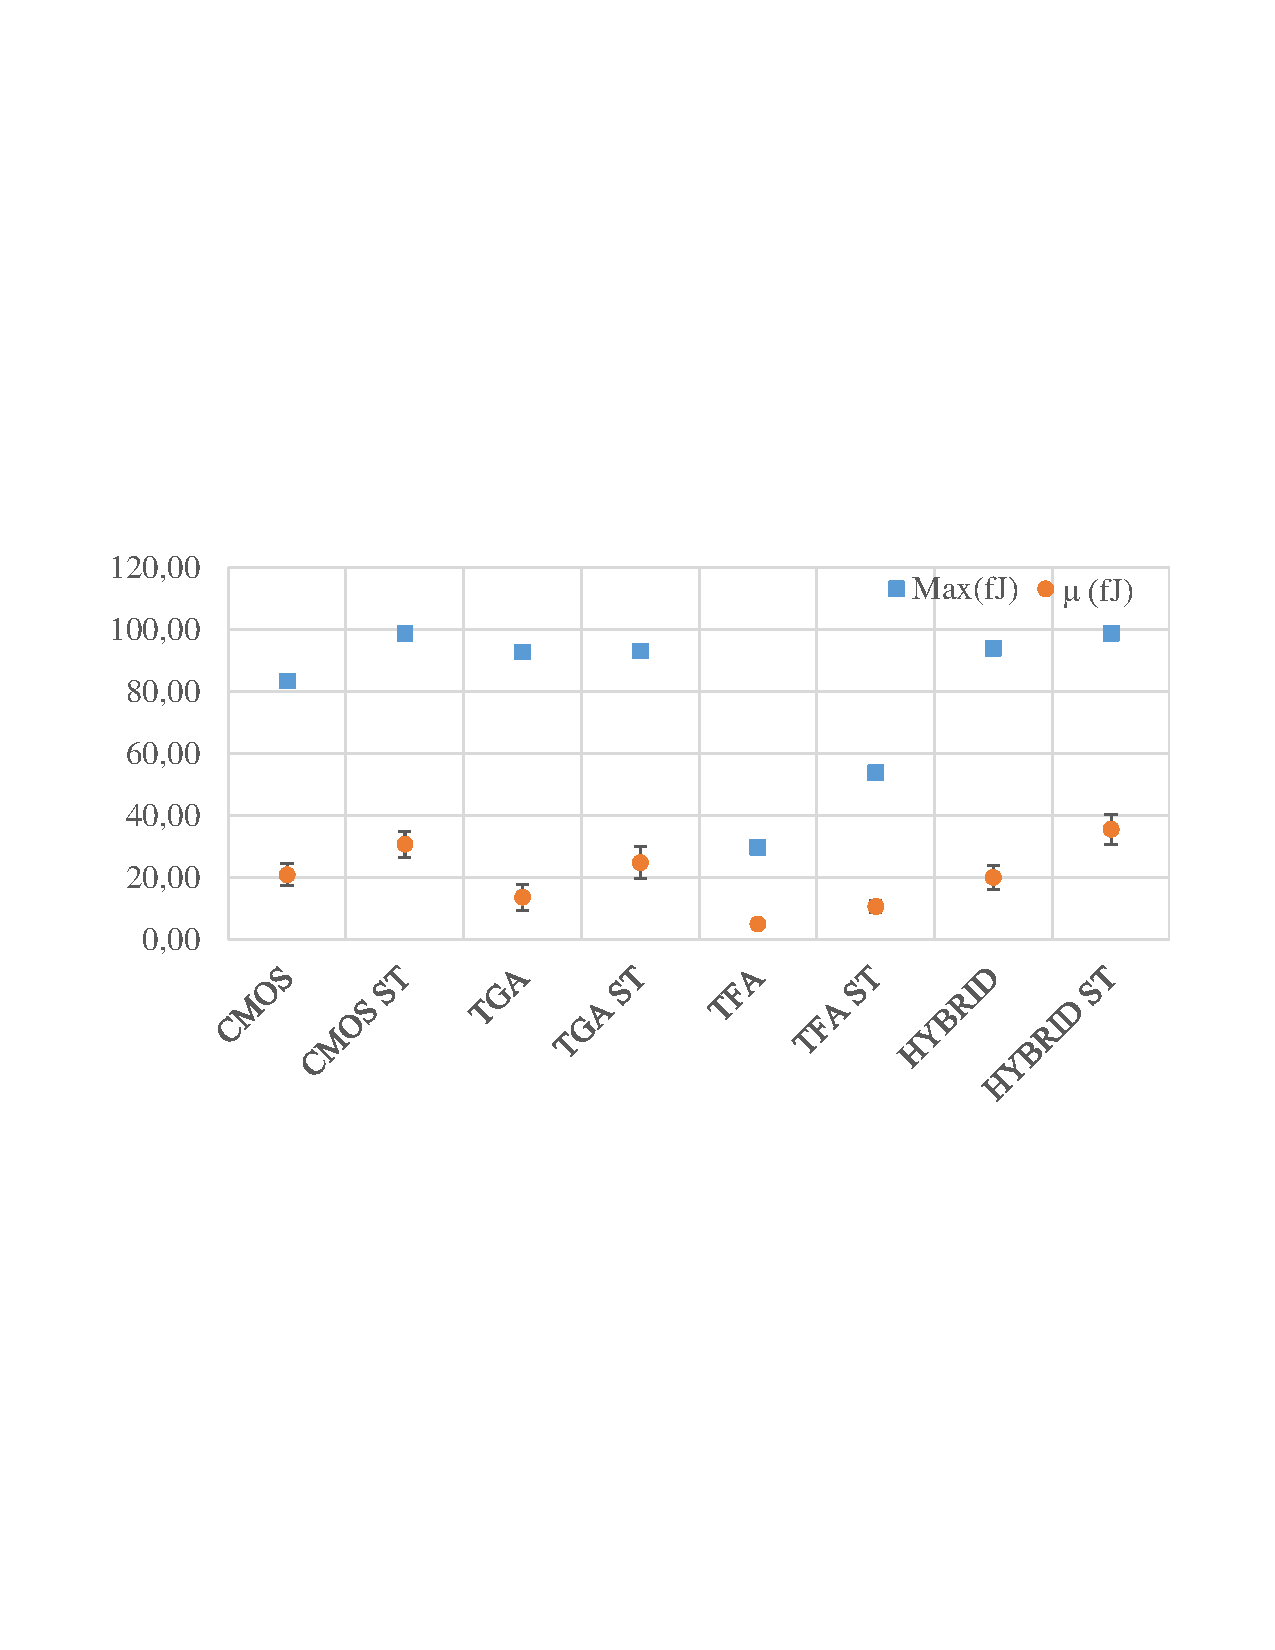
\includegraphics[width=\textwidth, trim={0 9cm 0 9cm},clip]{energyNominalCarryOut.pdf}
\caption{Energy measures for Carry Out output at nominal operation.}
\label{fig:Fig48}
%\legend{Source: \cite{dokania2015circuit}}
\end{figure}

\begin{figure}[H]
\centering
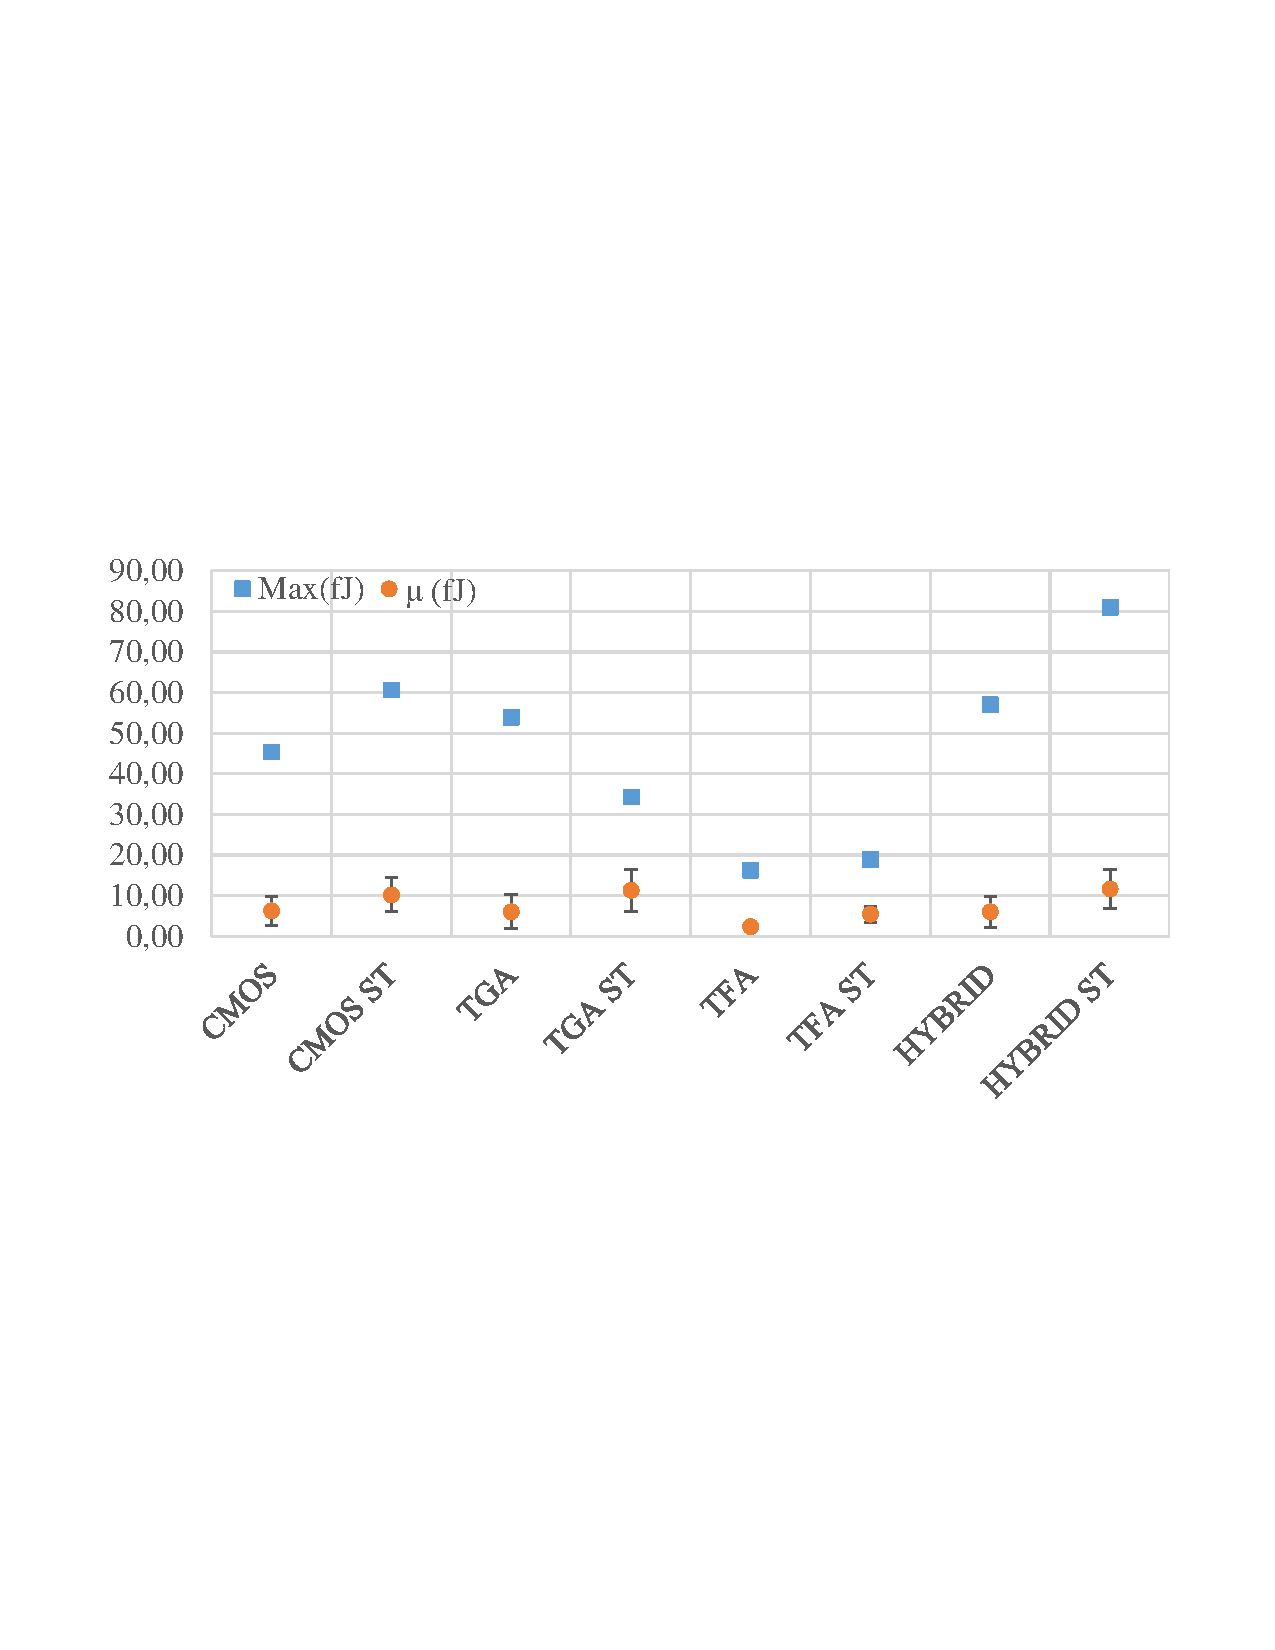
\includegraphics[width=\textwidth, trim={0 9cm 0 9cm},clip]{energyNTSum.pdf}
\caption{Energy measures for Sum output at near-threshold operation.}
\label{fig:Fig49}
%\legend{Source: \cite{dokania2015circuit}}
\end{figure}

\begin{figure}[H]
\centering
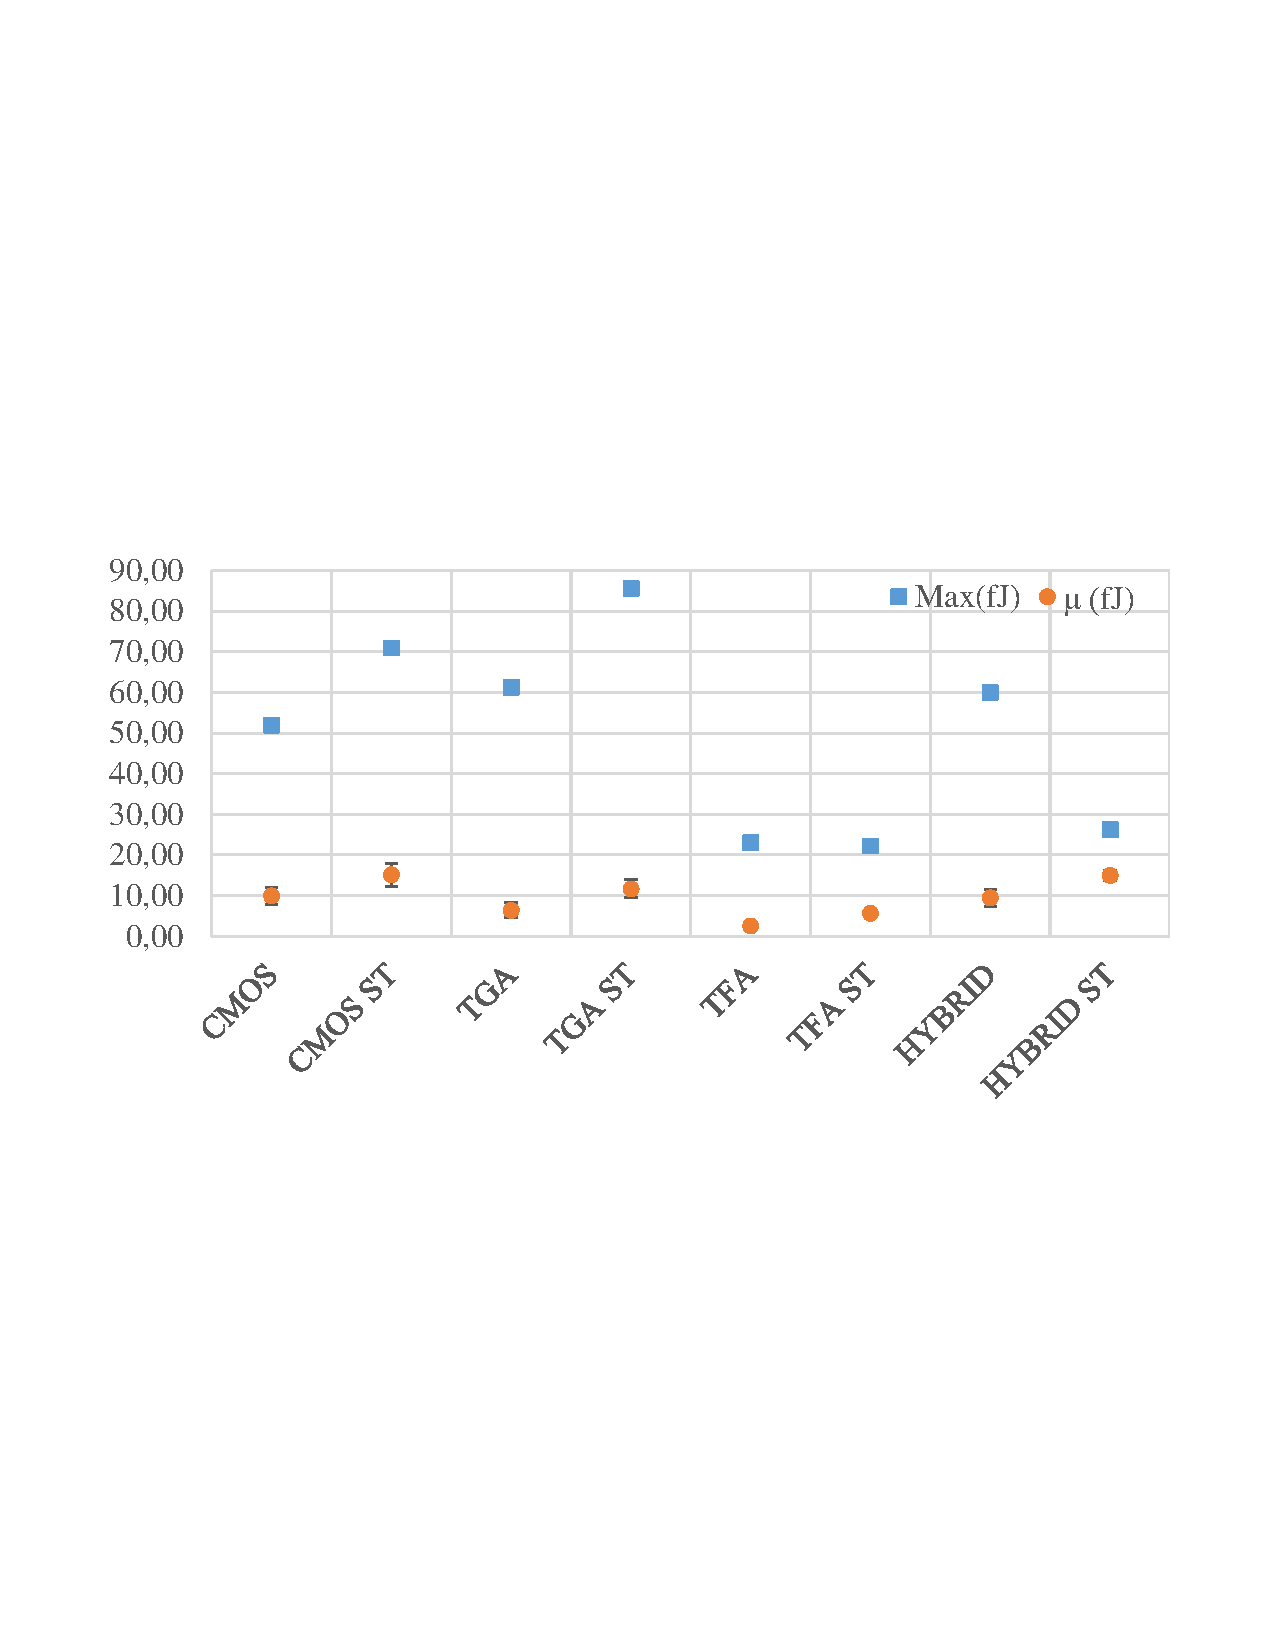
\includegraphics[width=\textwidth, trim={0 9cm 0 9cm},clip]{energyNTCarryOut.pdf}
\caption{Energy measures for Carry Out output at near-threshold operation.}
\label{fig:Fig410}
%\legend{Source: \cite{dokania2015circuit}}
\end{figure}

\begin{table}[H]
\centering
\caption{My caption}
\label{my-label}
\resizebox{\textwidth}{!}{%
\begin{tabular}{|l|r|r|r|r|c|r|r|r|r|c|}
\hline
\multicolumn{11}{|c|}{{\ul \textbf{SUM}}} \\ \hline
\multirow{2}{*}{\textbf{Full Adder}} & \multicolumn{5}{c|}{\textbf{Nominal @ 0.7V}} & \multicolumn{5}{c|}{\textbf{Near-threshold @ 0.4V}} \\ \cline{2-11} 
 & \multicolumn{1}{c|}{Max (ps)} & \multicolumn{1}{c|}{\mu (ps)} & \multicolumn{1}{c|}{\sigma (ps)} & \multicolumn{1}{c|}{\sigma/\mu (\%)} & \Delta(\%) & \multicolumn{1}{c|}{Max (ps)} & \multicolumn{1}{c|}{\mu (ps)} & \multicolumn{1}{c|}{\sigma (ps)} & \multicolumn{1}{c|}{\sigma/\mu (\%)} & \Delta(\%) \\ \hline
CMOS & 93.19 & 16.11 & 3.83 & 0.23 & \multirow{2}{*}{4.46} & 873.41 & 73.22 & 56.38 & 0.77 & \multirow{2}{*}{18.70} \\ \cline{1-5} \cline{7-10}
CMOS ST & 117.19 & 21.98 & 4.98 & 0.22 &  & 430.85 & 95.85 & 60.57 & 0.63 &  \\ \hline
TGA & 63.13 & 14.51 & 3.28 & 0.28 & \multirow{2}{*}{-11.65} & 7328.30 & 62.90 & 92.17 & 1.33 & \multirow{2}{*}{31.53} \\ \cline{1-5} \cline{7-10}
TGA ST & 77.71 & 17.63 & 3.80 & 0.31 &  & 2386.40 & 127.54 & 106.22 & 0.91 &  \\ \hline
TFA & 1016.90 & 12.63 & 10.62 & 0.59 & \multirow{2}{*}{37.43} & 1024.90 & 67.28 & 93.48 & 2.89 & \multirow{2}{*}{64.74} \\ \cline{1-5} \cline{7-10}
TFA ST & 83.52 & 15.39 & 4.16 & 0.37 &  & 4202.20 & 84.34 & 79.51 & 1.02 &  \\ \hline
HYBRID & 117.57 & 18.15 & 4.42 & 0.24 & \multirow{2}{*}{-0.75} & 830.64 & 95.23 & 77.95 & 0.79 & \multirow{2}{*}{13.43} \\ \cline{1-5} \cline{7-10}
HYBRID ST & 192.48 & 25.92 & 6.55 & 0.24 &  & 1212.00 & 120.92 & 86.26 & 0.68 &  \\ \hline
\end{tabular}%
}
\end{table}

\begin{table}[H]
\centering
\caption{My caption}
\label{my-label}
\resizebox{\textwidth}{!}{%
\begin{tabular}{|l|r|r|r|r|c|r|r|r|r|c|}
\hline
\multicolumn{11}{|c|}{{\ul \textbf{CARRY OUT}}} \\ \hline
\multirow{2}{*}{\textbf{Full Adder}} & \multicolumn{5}{c|}{\textbf{Nominal @ 0.7V}} & \multicolumn{5}{c|}{\textbf{Near-threshold @ 0.4V}} \\ \cline{2-11} 
 & \multicolumn{1}{c|}{Max (ps)} & \multicolumn{1}{c|}{\mu (ps)} & \multicolumn{1}{c|}{\sigma (ps)} & \multicolumn{1}{c|}{\sigma/\mu (\%)} & \Delta(\%) & \multicolumn{1}{c|}{Max (ps)} & \multicolumn{1}{c|}{\mu (ps)} & \multicolumn{1}{c|}{\sigma (ps)} & \multicolumn{1}{c|}{\sigma/\mu (\%)} & \Delta(\%) \\ \hline
CMOS & 104.48 & 27.38 & 5.92 & 0.22 & \multirow{2}{*}{1.05} & 794.87 & 128.65 & 86.67 & 0.67 & \multirow{2}{*}{11.61} \\ \cline{1-5} \cline{7-10}
CMOS ST & 120.01 & 33.09 & 7.08 & 0.21 &  & 539.77 & 143.77 & 85.67 & 0.60 &  \\ \hline
TGA & 60.11 & 16.32 & 4.28 & 0.29 & \multirow{2}{*}{15.77} & 6396.90 & 325.25 & 138.02 & 1.74 & \multirow{2}{*}{-19.14} \\ \cline{1-5} \cline{7-10}
TGA ST & 71.82 & 21.19 & 4.77 & 0.24 &  & 6265.10 & 181.01 & 373.37 & 2.07 &  \\ \hline
TFA & 2010.20 & 14.74 & 13.77 & 0.78 & \multirow{2}{*}{-25.64} & 5734.20 & 151.02 & 286.55 & 2.27 & \multirow{2}{*}{-21.16} \\ \cline{1-5} \cline{7-10}
TFA ST & 2030.50 & 22.72 & 37.42 & 0.97 &  & 6705.80 & 94.87 & 233.09 & 2.76 &  \\ \hline
HYBRID & 65.29 & 17.30 & 4.18 & 0.26 & \multirow{2}{*}{4.20} & 695.28 & 78.00 & 56.73 & 0.74 & \multirow{2}{*}{19.48} \\ \cline{1-5} \cline{7-10}
HYBRID ST & 96.40 & 23.27 & 5.64 & 0.25 &  & 2755.30 & 168.92 & 100.34 & 0.60 &  \\ \hline
\end{tabular}%
}
\end{table}

\begin{table}[H]
\centering
\caption{My caption}
\label{my-label}
\resizebox{\textwidth}{!}{%
\begin{tabular}{|l|r|r|r|r|c|r|r|r|r|c|}
\hline
\multicolumn{11}{|c|}{{\ul \textbf{SUM}}} \\ \hline
\multirow{2}{*}{\textbf{Full Adder}} & \multicolumn{5}{c|}{\textbf{Nominal @ 0.7V}} & \multicolumn{5}{c|}{\textbf{Near-threshold @ 0.4V}} \\ \cline{2-11} 
 & \multicolumn{1}{c|}{Max (fJ)} & \multicolumn{1}{c|}{\mu (fJ)} & \multicolumn{1}{c|}{\sigma (fJ)} & \multicolumn{1}{c|}{\sigma/\mu (\%)} & \Delta(\%) & \multicolumn{1}{c|}{Max (fJ)} & \multicolumn{1}{c|}{\mu (fJ)} & \multicolumn{1}{c|}{\sigma (fJ)} & \multicolumn{1}{c|}{\sigma/\mu (\%)} & \Delta(\%) \\ \hline
CMOS & 69.07 & 12.89 & 2.97 & 0.23 & \multirow{2}{*}{18.21} & 45.37 & 6.29 & 2.00 & 0.32 & \multirow{2}{*}{20.07} \\ \cline{1-5} \cline{7-10}
CMOS ST & 93.07 & 20.26 & 3.81 & 0.19 &  & 60.64 & 10.22 & 2.60 & 0.25 &  \\ \hline
TGA & 60.36 & 11.78 & 2.36 & 0.20 & \multirow{2}{*}{3.71} & 53.90 & 6.06 & 2.01 & 0.33 & \multirow{2}{*}{61.45} \\ \cline{1-5} \cline{7-10}
TGA ST & 90.61 & 22.99 & 4.44 & 0.19 &  & 34.33 & 11.30 & 1.44 & 0.13 &  \\ \hline
TFA & 21.94 & 4.45 & 0.92 & 0.21 & \multirow{2}{*}{33.73} & 16.26 & 2.40 & 0.65 & 0.27 & \multirow{2}{*}{66.59} \\ \cline{1-5} \cline{7-10}
TFA ST & 29.28 & 10.59 & 1.45 & 0.14 &  & 18.85 & 5.45 & 0.49 & 0.09 &  \\ \hline
HYBRID & 86.45 & 12.99 & 3.63 & 0.28 & \multirow{2}{*}{37.38} & 56.96 & 6.02 & 2.29 & 0.38 & \multirow{2}{*}{27.06} \\ \cline{1-5} \cline{7-10}
HYBRID ST & 87.13 & 23.67 & 4.15 & 0.18 &  & 81.05 & 11.65 & 3.23 & 0.28 &  \\ \hline
\end{tabular}%
}
\end{table}

\begin{table}[H]
\centering
\caption{My caption}
\label{my-label}
\resizebox{\textwidth}{!}{%
\begin{tabular}{|l|r|r|r|r|c|r|r|r|r|c|}
\hline
\multicolumn{11}{|c|}{{\ul \textbf{CARRY OUT}}} \\ \hline
\multirow{2}{*}{\textbf{Full Adder}} & \multicolumn{5}{c|}{\textbf{Nominal @ 0.7V}} & \multicolumn{5}{c|}{\textbf{Near-threshold @ 0.4V}} \\ \cline{2-11} 
 & \multicolumn{1}{c|}{Max (fJ)} & \multicolumn{1}{c|}{\mu (fJ)} & \multicolumn{1}{c|}{\sigma (fJ)} & \multicolumn{1}{c|}{\sigma/\mu (\%)} & \Delta(\%) & \multicolumn{1}{c|}{Max (fJ)} & \multicolumn{1}{c|}{\mu (fJ)} & \multicolumn{1}{c|}{\sigma (fJ)} & \multicolumn{1}{c|}{\sigma/\mu (\%)} & \Delta(\%) \\ \hline
CMOS & 83.43 & 20.88 & 3.52 & 0.17 & \multirow{2}{*}{18.91} & 51.91 & 9.97 & 2.09 & 0.21 & \multirow{2}{*}{12.02} \\ \cline{1-5} \cline{7-10}
CMOS ST & 98.66 & 30.69 & 4.20 & 0.14 &  & 70.97 & 15.16 & 2.80 & 0.18 &  \\ \hline
TGA & 92.71 & 13.54 & 4.15 & 0.31 & \multirow{2}{*}{31.32} & 61.28 & 6.40 & 1.85 & 0.29 & \multirow{2}{*}{34.04} \\ \cline{1-5} \cline{7-10}
TGA ST & 93.03 & 24.79 & 5.21 & 0.21 &  & 85.49 & 11.67 & 2.22 & 0.19 &  \\ \hline
TFA & 29.74 & 4.96 & 1.14 & 0.23 & \multirow{2}{*}{19.62} & 23.03 & 2.58 & 0.64 & 0.25 & \multirow{2}{*}{52.18} \\ \cline{1-5} \cline{7-10}
TFA ST & 53.74 & 10.58 & 1.96 & 0.18 &  & 22.21 & 5.61 & 0.66 & 0.12 &  \\ \hline
HYBRID & 93.88 & 19.99 & 3.89 & 0.19 & \multirow{2}{*}{29.74} & 59.99 & 9.46 & 2.00 & 0.21 & \multirow{2}{*}{61.91} \\ \cline{1-5} \cline{7-10}
HYBRID ST & 98.85 & 35.58 & 4.87 & 0.14 &  & 26.22 & 15.03 & 1.21 & 0.08 &  \\ \hline
\end{tabular}%
}
\end{table}

\section{Penalties}
It is expected that a technique which replaces a 2-transistor sub-circuit to a 4-transistor one should bring an impact over metrics. Given so, the average impact at nominal operation was 30\% over delays and their absolute deviations. For energy, the impact is considerable, being on average over 85\% percent higher energy consumption. For energy standard deviations there was a 40\% increase at nominal level and a minor 4\% increase at near-threshold level. An overview of the penalties is shown at Figures K and J and…
For area penalties there was 250\%, 287.5\%, 200\% and 307\% increase for the CMOS, TGA, TFA and Hybrid Full Adders, respectively. Their respective areas are shown at Table 1. Such high area penalties are mainly due to technology rules such as the 108nm well-spacing and the necessity to use TAP-Cells to explicitly connect the transistors bulk to specific parts of the circuits or the supply/ground making the ST cell much bigger than expected. The Full Adders layouts are show at Figures C, K, L…

\begin{table}[H]
\centering
\caption{My caption}
\label{my-label}
\begin{tabular}{|l|l|l|}
\hline
\textbf{Full Adder} & \textbf{Area ($2^{\mu m}$)} & \textbf{Ratio} \\ \hline
CMOS & 0.34 & \multirow{2}{*}{2.5} \\ \cline{1-2}
CMOS ST & 0.85 &  \\ \hline
TGA & 0.54 & \multirow{2}{*}{2.875} \\ \cline{1-2}
TGA ST & 1.56 &  \\ \hline
TFA & 0.47 & \multirow{2}{*}{2} \\ \cline{1-2}
TFA ST & 0.95 &  \\ \hline
HYBRID & 0.51 & \multirow{2}{*}{3.07} \\ \cline{1-2}
HYBRID ST & 1.56 &  \\ \hline
\end{tabular}
\end{table}

\begin{figure}[H]
\centering
\begin{subfigure}[b]{\textwidth}
   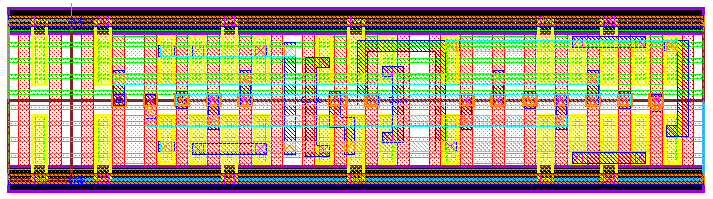
\includegraphics[width=1\linewidth]{CMOS.png}
   \caption{}
   \label{fig:Ng1} 
\end{subfigure}

\begin{subfigure}[b]{\textwidth}
   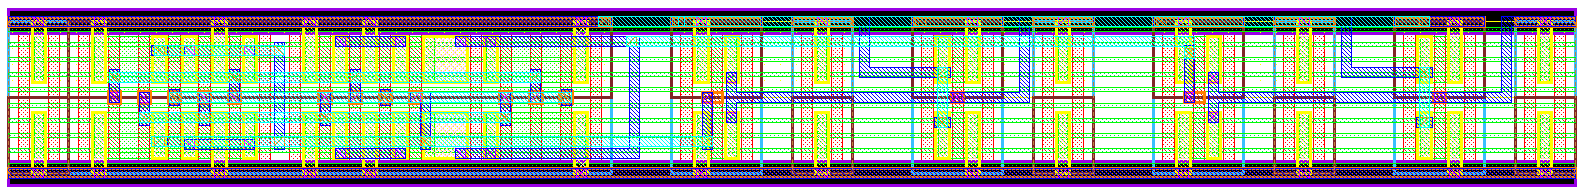
\includegraphics[width=1\linewidth]{CMOSST.png}
   \caption{}
   \label{fig:Ng2}
\end{subfigure}

\caption{}
\end{figure}

\begin{figure}[H]
\centering
\begin{subfigure}[b]{\textwidth}
   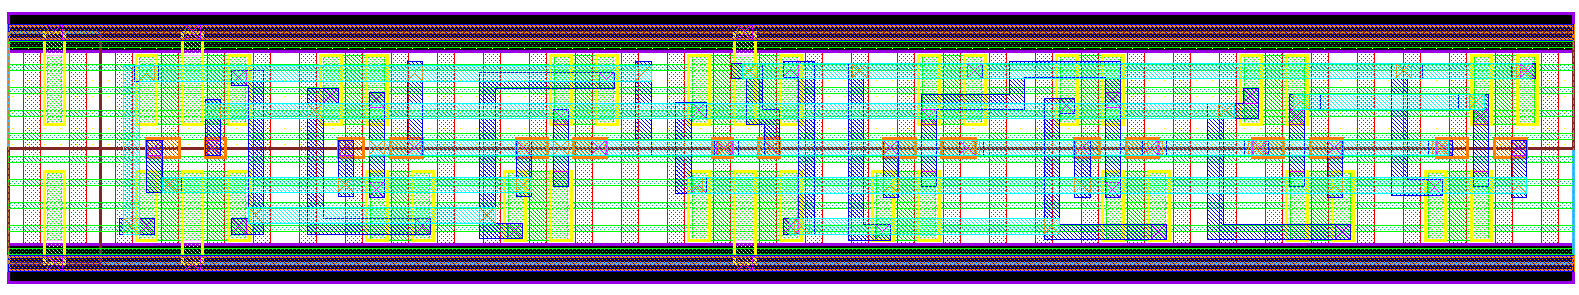
\includegraphics[width=1\linewidth]{TGA.png}
   \caption{}
   \label{fig:Ng1} 
\end{subfigure}

\begin{subfigure}[b]{\textwidth}
   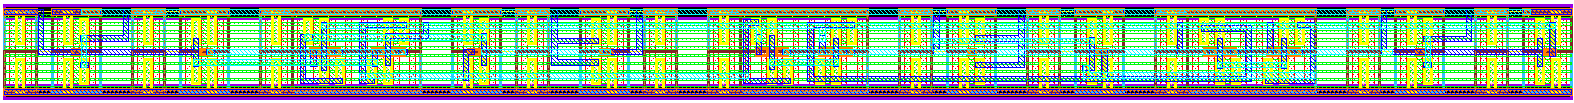
\includegraphics[width=1\linewidth]{TGAST.png}
   \caption{}
   \label{fig:Ng2}
\end{subfigure}

\caption{}
\end{figure}

\begin{figure}[H]
\centering
\begin{subfigure}[b]{\textwidth}
   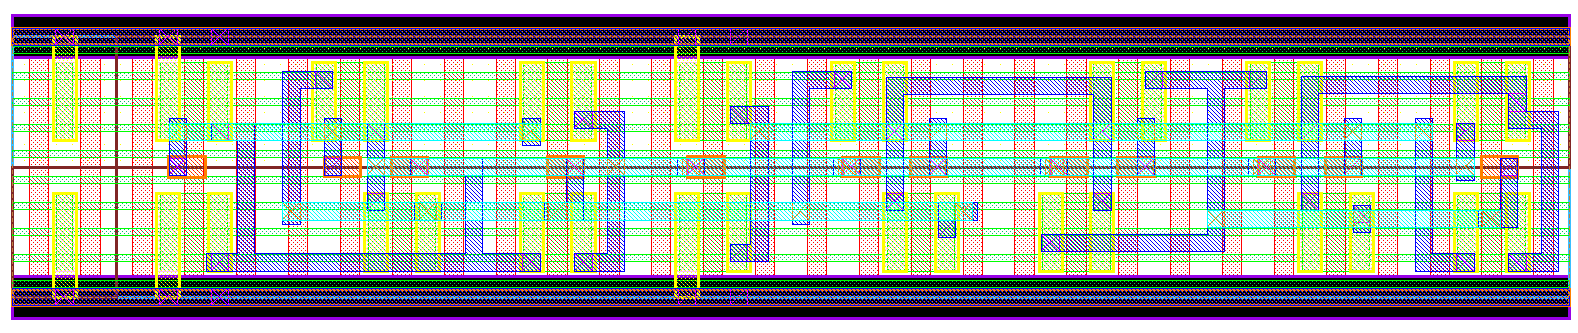
\includegraphics[width=1\linewidth]{TFA.png}
   \caption{}
   \label{fig:Ng1} 
\end{subfigure}

\begin{subfigure}[b]{\textwidth}
   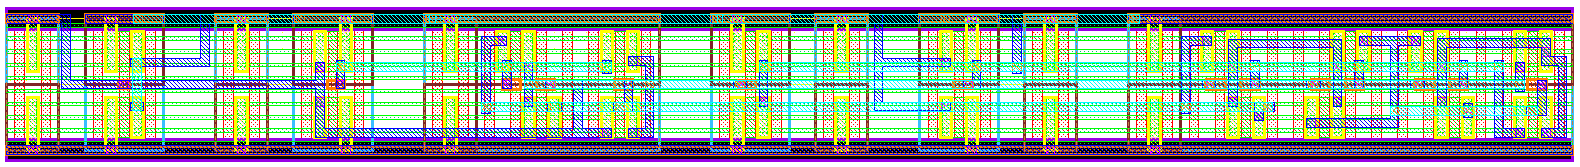
\includegraphics[width=1\linewidth]{TFAST.png}
   \caption{}
   \label{fig:Ng2}
\end{subfigure}

\caption{}
\end{figure}

\begin{figure}[H]
\centering
\begin{subfigure}[b]{\textwidth}
   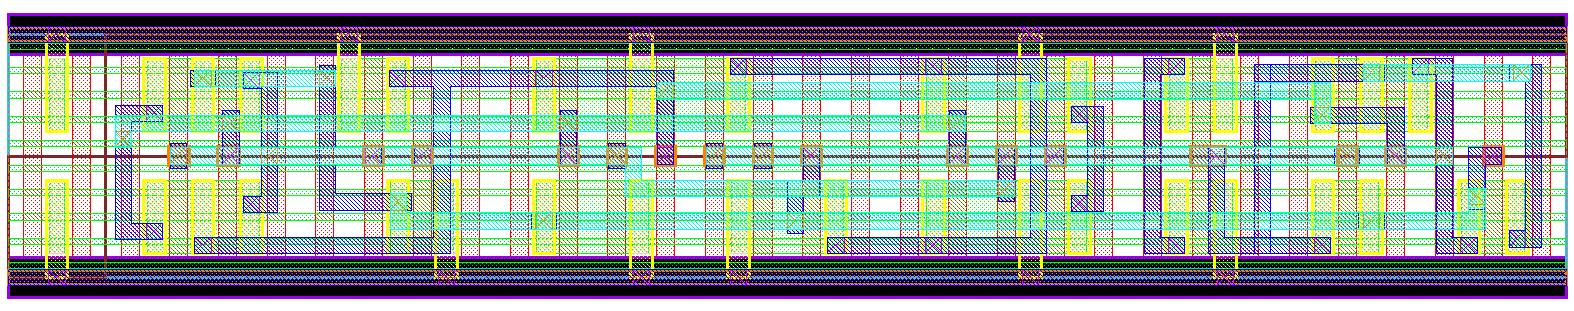
\includegraphics[width=1\linewidth]{HYBRID.png}
   \caption{}
   \label{fig:Ng1} 
\end{subfigure}

\begin{subfigure}[b]{\textwidth}
   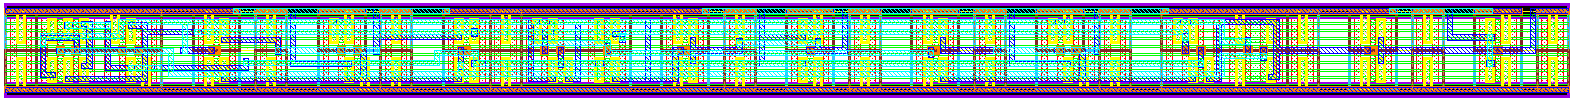
\includegraphics[width=1\linewidth]{HYBRIDST.png}
   \caption{}
   \label{fig:Ng2}
\end{subfigure}

\caption{}
\end{figure}

\chapter{Conclusions}
Variability has been a critical challenge in emerging technology nodes. Deviating the correct circuit’s behavior and affecting manufacturing yield. All current work in developing and validating techniques have been done at electrical and transistor level. There is a need of novel techniques which to improve variability robustness at layout and physical level.

Given that, a novel technique is tested. The technique consists of replacing internal inverters with Schmitt Trigger inverters in order to increase the circuit’s noise-immunity. As results show, the technique improves, sometimes drastically, the energy variability robustness for each Full Adder considered. For delay robustness, in some cases, there was a worsening in robustness mainly caused by area penalty and the pass-transistor logic.

With the technique penalties in mind, it should only be utilized in applications that can bear the delays, energy consumption and area increase with variability robustness as a priority. This works demonstrates the need for new techniques at layout level to address variability for high performance/low power applications with low area penalties

It is important to note that, according to the state-of-art research, this is the first analysis of this technique made at layout level. For future works, a supply voltage calibration shall be made to find the best cost-benefit supply voltage.   


\bibliographystyle{abntex2-alf}
\bibliography{biblio}

\end{document}
